
\Qsec{1}{Принцип Ферма}


\Ssec{6}{Предельный переход от волновой оптики к геометрической}
\input{parts/S06}


\Qsec{6}{Дисперсия волн}


\Ssec{10}{(k) Дисперсия}
\subsection{Дисперсия}

\textbf{Фазовая скорость}. 
В терминах фазовой скорости можно записать, что
\begin{equation*}
    u(x, t) = a\cos(kx-\omega t) = a \cos\left[k(x- \sub{v}{ф} t)\right],
\end{equation*}
то есть со скоростью $\sub{v}{ф}$ перемещается точка волны, фаза которой имеет фиксированной значение: $\varphi(x, t) = \omega  t - k x = \const$. В общем случае связь частоты и волнового числа определяется законом дисперсии $\omega = \omega(k) = \omega(\lambda)$. 



\begin{to_def}
    \textit{Фазовой скоростью} называют величину $\sub{v}{ф} = \omega/k = c/n$.
\end{to_def}


\begin{to_def}
    Зависимость фазовой скорости от длины волны -- \textit{дисперсия}.
\end{to_def}



\textbf{Групповая скорость}. Рассмотрим две волны со скоростями $\omega_1$ и $\omega_2$ с соответсвующими $k_1(\omega_1)$ и $k_2(\omega_2)$. Пусть волны задаются уравнениями
\begin{equation*}
    \left.\begin{aligned}
        u_1 &= a \sin (k_1 x - \omega_1 t) \\
        u_2 &= a \sin(k_2 x - \omega_2 t)
    \end{aligned}\right.
    \hspace{0.5cm} \Rightarrow \hspace{0.5cm}
    u(x, t) = u_1 + u_2 = 2 a \cos\left[
        \frac{k_2-k_1}{2}x - \frac{\omega_2-\omega_1}{2}t
    \right] \sin\left[
        \frac{k_2 + k_1}{2}x - \frac{\omega_2+\omega_1}{2}t
    \right].
\end{equation*}
Логично ожидать, что $k_2-k_1 \ll k_1$, тогда считая $k = \langle k_1,\,  k_2\rangle$,  $\omega = \langle \omega_1,\, \omega_2\rangle$ и $k_2 - k_1 = \Delta k$, $\omega_2-\omega_1 = \frac{d \omega}{d k} \Delta k$, перепишем выражение в виде
\begin{equation*}
    u(x, t) = 2 a \cos\left[
        \frac{\Delta k}{2} \left(
            x - \frac{d \omega}{d k} t
        \right)
    \right] \cdot \sin(kx - \omega t),
\end{equation*}
что очень сильно напоминает биения. Получается, что рассматривая эволюцию волны во времени корректно ввести \textit{групповую скорость} $\sub{v}{гр} = \d\omega/\d k$, -- при таком движении модуляция волны сохраняет фиксированное значение. Это обобщается и на некоторый диапазон $k_i$, тогда получим выражение вида
\begin{equation*}
    u(x, t) = \exp\left[i(kx-\omega t)\right] F(x- \sub{v}{гр}t).
\end{equation*}
Именно с функцией $F(x- \sub{v}{гр}t)$ связывают представление о цуге волн, или \textit{волновом пакете}. 


\textbf{Формула Рэлея}. Найдём связь фазовой и групповой скоростей: считая $\omega = k \sub{v}{ф}$ находим сотношение вида
\begin{equation*}
    \sub{v}{гр} = \sub{v}{ф} - \lambda \frac{d \sub{v}{ф}}{d \lambda}, 
\end{equation*} 
которое называют \textit{формулой Рэлея}. 

Свяжем групповую скорость волны с показателем преломления. Из формулы Рэлея:
\begin{equation*}
    \sub{v}{гр} = \sub{v}{ф} - \lambda \frac{d }{d \lambda} \left(\frac{c}{n}\right) = 
    \sub{v}{ф} \left(1 + \frac{\lambda}{n} \frac{d n}{d \lambda} \right) = 
    \frac{c}{n + \omega \ d n / \d \omega}
    .
\end{equation*}
Однако также верно, что $\lambda = \frac{2 \pi c}{n \omega}$, так что корректнее иметь производну. по частоте. 



\textbf{Нормальная и аномальная дисперсия}. Пусть $\sqrt{\varepsilon} = n + i \kappa$. Величина $n = \Re\sqrt{\varepsilon}$ -- \textit{показатель преломления}, и $\kappa = \Im \sqrt{ \varepsilon}$ -- \textit{показатель поглощения} (затухания). 


Представляя атомы осцилляторами с собственной частотой $\omega_0 = \sqrt{\beta/m}$ и коэффициентом затухания $\gamma = \eta/2m$ можно для концентрации атомов $N$ найти проницаемость
\begin{equation*}
    \varepsilon = 1 + \frac{\omega_p^2}{\omega_0^2 - \omega^2 - 2 i \gamma \omega}, \hspace{5 mm} 
    \omega_p^2 = 4 \pi N \frac{e^2}{m}. 
\end{equation*}
Вообще можно выделить нормальну ($n'_\omega > 0$) и аномальную ($n'_\omega < 0$) дисперсию, подробнее на рис. \ref{fig:abn}. 
\begin{figure}[h]
    \centering
    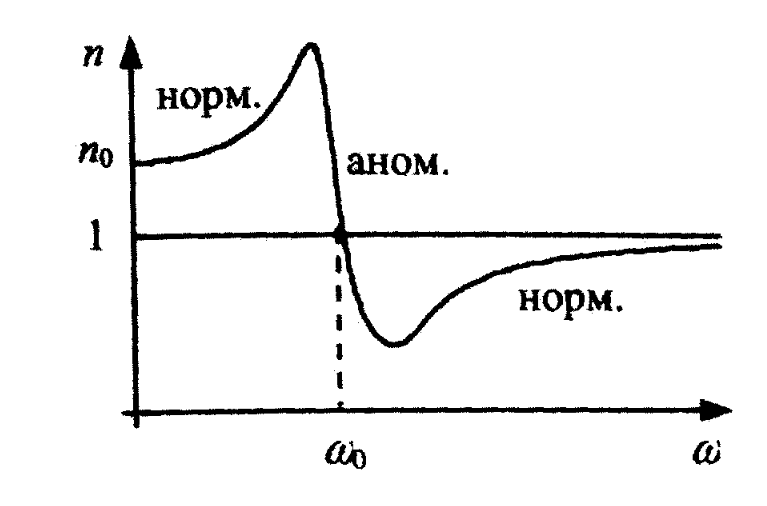
\includegraphics[width=0.3\textwidth]{figures/k10_1.png}
    \caption{Аномальная и нормальная дисперсия}
    \label{fig:abn}
\end{figure}
Для случая, когда $\varepsilon(\omega)$ не сильно отличается от $1$, можно получить следующие выражения
\begin{equation*}
    n = 1 + \frac{\omega_p^2}{2} \frac{\omega_0^2-\omega^2}{(\omega_0^2-\omega^2)^2 + 4 \gamma^2 \omega^2}, \hspace{5 mm} 
    \kappa = \frac{\gamma \omega_p^2 \omega}{(\omega_0^2-\omega^2)^2+4 \gamma^2 \omega^2}.
\end{equation*}


\textbf{Закон Бугера}. Чуть подробнее раскрывая показатель поглощения:
\begin{equation*}
    k = \frac{\omega}{c} \sqrt{\varepsilon} = \frac{\omega}{c} n + i \frac{\omega}{c}\kappa,
\end{equation*}
где вводится $\alpha = \frac{4\pi}{\lambda_0} \kappa$ и $\lambda_0 = \frac{2 \pi c}{\omega}$ -- длина волны излучения в вакууме на частоте $\omega$. Итого, для бегущей волны получается
\begin{equation*}
    E \sim e^{ik_r x} e^{- \alpha x/2},
    \hspace{0.5cm} \Rightarrow \hspace{0.5cm}
    I = I_0 e^{- \alpha x},
\end{equation*}
что и называют \textit{законом Бугера}. 





\textbf{Закон Лоренца-Лоренца}. Когда велика концентрация свободных электронов значимым становится поле электронов, действующее на остальные, что может быть сравнимо с действием внешнего поля. Так можем связать $\varepsilon$ и поляризуемость отдельных молекцл $\beta$ 
\begin{equation*}
    \varepsilon = \frac{1 + \frac{8\pi}{3} N \beta}{1 - \frac{4\pi}{3} N \beta},
    \hspace{0.5cm} \Rightarrow \hspace{0.5cm}   
    \frac{4 \pi}{3} N \beta = \frac{\varepsilon-1}{\varepsilon+1},
\end{equation*}
что называют \textit{формулой Лоренца-Лоренца}. 






\Ssec{87}{Дисперсия плазмы}
\subsection{Дисперсия плазмы}


\textbf{Плазменная частота}. Можно написать штуку из \S 84, но ненужно. 
Если атомы колеблются на $\omega_0$, частоты волны $\omega$, концентрация атомов в единице объема $N$, масса атомов $m$, $\gamma$ -- ну, какая-то гамма для затухания, то можем прийти к формуле
\begin{equation*}
    \varepsilon = 1 + \frac{4 \pi N e^2/m}{\omega_0^2 - \omega^2 + 2 i w \gamma},
\end{equation*}
где последнее слагаемое как раз характеризует поляризуемость атома. 
На самом деле достаточно рассмотреть а-ля конденсатор в плазме, как в прошлом семестре. 

Диэлектрическая проницаемость плазмы определяется в основном \textit{свободными электронами}. Полагая $\omega_0 = 0$, пренебрегая затуханием ($\gamma=0$), получаем для плазмы
\begin{equation*}
    \varepsilon = 1 - \left(\frac{\omega_p}{\omega}\right)^2,
    \hspace{5 mm} 
    \omega_p^2 = 4 \pi N\frac{e^2}{m},
\end{equation*}
где $N$ -- концентрация свободных электронов. Величина $\omega_p$ -- \textit{плазменная}, или \textit{ленгмюровская} частота, играющая для плазмы роль \textit{собственной частоты}. 



При $\omega < \omega_p$ $\varepsilon < 0$, так что длинные эм волны отражаются от плазмы. Эксплуатируя этот эффект можем реализовать дальнюю радиосвязь: на земле $N$ меняется с высотой неравномерно, есть несколько максимумов, и область с одним из таких максимумов и называется ионосферным слоем. Характерные значения для $N \in [10^4; 10^6]$ электронов на $1$ см$^3$. 


\textbf{Фазовая и групповая скорость}. Для волнового числа можем записать
\begin{equation*}
    c^2 k^2 = \omega^2 \varepsilon = \omega^2 - \omega^2_p,
    \hspace{0.5cm} \Rightarrow \hspace{0.5cm}   
    c^2 k \d k = \omega \d \omega,
    \hspace{0.5cm} \Rightarrow \hspace{0.5cm}
    \frac{\omega}{k} \frac{d \omega}{d k}  = c^2,
\end{equation*}
иначе можем записать, как
\begin{equation*}
    v u = c^2, \hspace{5 mm} 
    v = \frac{c}{\sqrt{\varepsilon}} = \frac{c}{\sqrt{1-\omega_p^2/\omega^2}} > c,
    \hspace{5 mm} 
    u = \frac{c^2}{v} = c \sqrt{1- \frac{\omega_p^2}{\omega^2}} < c.
\end{equation*}
Соответственно, некоторый важный итог:
\begin{equation*}
    n = \frac{c}{v} = \sqrt{1- \frac{\omega_p^2}{\omega}}, \hspace{5 mm} 
    \omega_p^2 = 4 \pi N \frac{e^2}{m}.
\end{equation*}

\Qsec{7}{Классическая теория дисперсии света и дисперсия в плазме}

\Ssec{87}{Дисперсия плазмы}
\subsection{Дисперсия плазмы}


\textbf{Плазменная частота}. Можно написать штуку из \S 84, но ненужно. 
Если атомы колеблются на $\omega_0$, частоты волны $\omega$, концентрация атомов в единице объема $N$, масса атомов $m$, $\gamma$ -- ну, какая-то гамма для затухания, то можем прийти к формуле
\begin{equation*}
    \varepsilon = 1 + \frac{4 \pi N e^2/m}{\omega_0^2 - \omega^2 + 2 i w \gamma},
\end{equation*}
где последнее слагаемое как раз характеризует поляризуемость атома. 
На самом деле достаточно рассмотреть а-ля конденсатор в плазме, как в прошлом семестре. 

Диэлектрическая проницаемость плазмы определяется в основном \textit{свободными электронами}. Полагая $\omega_0 = 0$, пренебрегая затуханием ($\gamma=0$), получаем для плазмы
\begin{equation*}
    \varepsilon = 1 - \left(\frac{\omega_p}{\omega}\right)^2,
    \hspace{5 mm} 
    \omega_p^2 = 4 \pi N\frac{e^2}{m},
\end{equation*}
где $N$ -- концентрация свободных электронов. Величина $\omega_p$ -- \textit{плазменная}, или \textit{ленгмюровская} частота, играющая для плазмы роль \textit{собственной частоты}. 



При $\omega < \omega_p$ $\varepsilon < 0$, так что длинные эм волны отражаются от плазмы. Эксплуатируя этот эффект можем реализовать дальнюю радиосвязь: на земле $N$ меняется с высотой неравномерно, есть несколько максимумов, и область с одним из таких максимумов и называется ионосферным слоем. Характерные значения для $N \in [10^4; 10^6]$ электронов на $1$ см$^3$. 


\textbf{Фазовая и групповая скорость}. Для волнового числа можем записать
\begin{equation*}
    c^2 k^2 = \omega^2 \varepsilon = \omega^2 - \omega^2_p,
    \hspace{0.5cm} \Rightarrow \hspace{0.5cm}   
    c^2 k \d k = \omega \d \omega,
    \hspace{0.5cm} \Rightarrow \hspace{0.5cm}
    \frac{\omega}{k} \frac{d \omega}{d k}  = c^2,
\end{equation*}
иначе можем записать, как
\begin{equation*}
    v u = c^2, \hspace{5 mm} 
    v = \frac{c}{\sqrt{\varepsilon}} = \frac{c}{\sqrt{1-\omega_p^2/\omega^2}} > c,
    \hspace{5 mm} 
    u = \frac{c^2}{v} = c \sqrt{1- \frac{\omega_p^2}{\omega^2}} < c.
\end{equation*}
Соответственно, некоторый важный итог:
\begin{equation*}
    n = \frac{c}{v} = \sqrt{1- \frac{\omega_p^2}{\omega}}, \hspace{5 mm} 
    \omega_p^2 = 4 \pi N \frac{e^2}{m}.
\end{equation*}



\Qsec{9}{Статистическая природа света}
\Ssec{31}{Корреляция и когерентность света}


\textbf{Квазимонохроматичность}. 
Если область $\Delta \omega$ в которую входит 
% $p.\, v.$
 основное значение интеграла Фурье, и $\Delta \omega / \omega \ll 1$, то результирующее колебание называется \textit{квазимонохроматическое}. Запишем произвольные квазимонохроматические колебания в виде
\begin{equation*}
    E(t) = a(t) e^{i \omega_0 t},
\end{equation*}
где $a(t)$ -- медленная амплитуда, таким образом колебания модулированы, меняется $a(t)$ -- амплитудная модуляция, меняется фаза -- \textit{фазовая модуляция}. 


Так как детекция происходит в основном для интенсивности, то про неё и будем гворить, квадрат поля может быть представлен в виде
\begin{equation*}
    (\Re E)^2 = \left(\frac{E + E^*}{2}\right)^2 = \frac{1}{4} \left(E^2 + E^{*2}\right) + \frac{1}{2} E E^*.
\end{equation*}
Если считать $a = a_0 (t) e^{i \delta(t)}$, где $a_0(t)$ и $\delta(t)$ -- межденно меняющиеся вещественная амплитуда и фаза, то
\begin{equation*}
    E^2 + E^{*2} = 2 a_0^2 \cos\left[2(\omega_0 r + \delta)\right],
\end{equation*}
что быстроосциллирует, так что $0$. Поэтому интенсивность $\langle E E^*\rangle$. 



\textbf{Два источника}.
Рассмотрим теперь сумму колебаний от двух источников из $S_1$ и $S_2$ с отставваиями на $\theta_1$ и $\theta_2$. Тогда результирующее 
\begin{equation*}
    E \equiv E(P, t) = E_1(t-\theta_1) + E_2 (t-\theta_2).
\end{equation*}
Умножая на комплексно-сопряженное и усредняя по времени приходим к выражению вида
\begin{equation*}
    I = I_1 + I_2 + 2 \sqrt{I_1 I_2} \Re\left[f_{12}(\theta)\right],
\end{equation*}
где $\theta = \theta_2-\theta_1$. 

\begin{to_def}
    \textit{Корреляционной функцией} колебаний $E_1(t-\theta_1)$ и $E_2(t-\theta_2)$ называют 
    \begin{equation*}
        \left\langle 
            E_1(t-\theta_1) E_2^* (t-\theta_2)
        \right\rangle = \left\langle E_1(t) E_2^* (t-\theta)\right\rangle = F_{1, 2}(\theta) = \sqrt{I_1 I_2}f_{1,2} (\theta).
    \end{equation*}
    Она характеризует степень согласованности колебаний. Функция $f_{1, 2}$ называется \textit{нормированной корреляционной функцией}. Разделив её на быстро осциллирующую функцию $e^{i \omega_0 t}$ можем перейти к \textit{комплексной степени когерености колебаний}
    \begin{equation*}
        \gamma_{1,2}(\theta) = f_{1, 2} (\theta) e^{-i \omega_0 \theta},
    \end{equation*}
    модуль которой -- степень когерентнсоти колебаний в точке $P$. 
\end{to_def}



Итого, в терминах $\gamma$, переходим к
\begin{equation*}
    I = I_1 + I_2 + 2 \sqrt{I_1 I_2} \Re\left[\gamma(\theta) e^{i \omega_0 \theta}\right] = 
    I_1 + I_2 + 2 \sqrt{I_1 I_2}  |\gamma_{1,2}(\theta)| \cos(\omega_0 \theta + \delta(\theta)),
\end{equation*}
где $\gamma_{1,2} (\theta) = |\gamma_{1, 2}|e^{i \delta}$. Однако $\gamma$ меняется медленно, так что в максимумах $\cos(\omega_0 \theta + \delta) = +1$ и в минимумах $\cos(\omega_0 \theta + \delta) = -1$, тогда
\begin{equation*}
    \sub{I}{max} = I_1 + I_2 + 2 \sqrt{I_1 I_2} |\gamma_{1, 2} (\theta)|,
    \hspace{5 mm} 
    \sub{I}{min} = I_1 + I_2 - 2 \sqrt{I_1 I_2} |\gamma_{1, 2} (\theta)|,
    \hspace{0.5cm} \Rightarrow \hspace{0.5cm}
    V \equiv \frac{\sub{I}{max}-\sub{I}{min}}{\sub{I}{max}+\sub{I}{min}} = \frac{2 \sqrt{I_1 I_2}}{I_1 + I_2} |\gamma_{1,2} (\theta)|.
\end{equation*}
Получается, что при $\gamma_{1, 2}(\theta) =0$ колеабния \textit{некогеренты}, и если $\gamma_{1, 2}(\theta) \equiv 0,\, \forall \theta$, то \textit{некогерентность полная}, тогда всюду имеет место \textit{закон фотометрического сложения}. 

Интереференция \textit{полная} при $\gamma_{1, 2}(\theta) \equiv 1$, такой случай реализуется при наложении строго
периодических, в частности монохроматических, пучков одинаковых периодов. Вопросы \textit{пространственной} и \textit{временной} когерентности колебаний некоторого поля могут быть сведены к рассмотрению $\gamma$ для ситуции рис. \ref{fig:31}.
\begin{figure}[h]
    \centering
    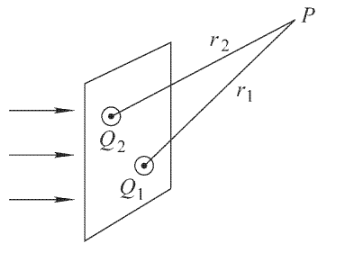
\includegraphics[width=0.27\textwidth]{figures/31_1.png}
    \caption{Расчёт пространственной и временной когерентности.}
    \label{fig:31}
\end{figure}


\textbf{Оборванная синусоида}. Пусть есть $\sin$ вплоть до некоторого $\tau$ по которому и будем усреднять
\begin{equation*}
    E(t) = \left\{\begin{aligned}
        &\sin \omega_0 t, &t \in[0, \tau], \\
        &0,     &t \notin [0, \tau],
    \end{aligned}\right.
    \hspace{0.5cm} \Rightarrow \hspace{0.5cm}
    \gamma(\theta) = \left\{\begin{aligned}
        &1-\theta/\tau, &\theta < \tau, \\
        &0, &\theta > \tau.
    \end{aligned}\right.
\end{equation*}
что может быть получено из выражения
\begin{equation*}
    \left\langle E(t) E^* (t-\theta)\right\rangle = \frac{1}{\tau} \int_0^\tau e^{i \omega_0 \theta} \d t = \frac{\tau-\theta}{\tau} e^{i \omega_0 \theta} = F(\theta) = f(\theta).
\end{equation*}


\textbf{Связь автокорреляционной функции и спектральной плотности}. Да, они связаны: $F(\theta)$ и $I_\omega(\omega)$. Для установления связи запишем по определению
\begin{equation*}
    F(\theta) = \left\langle E(t) E^* (t-\theta)\right\rangle = \frac{1}{\tau} \int_{-\tau/2}^{\tau/2} E(t) E^* (t-\theta) \d t,
\end{equation*}
подтсавляя $E^*(t-\theta) = \int_0^\infty a^* (\omega) e^{-i \omega (t-\theta)} \d \omega$, а также вспоминая выражения для $a(\omega)$, и меняя порядок интегрирования приходим к
\begin{equation*}
    a(\omega) = \frac{1}{2\pi} \int_{-\tau/2}^{\tau/2} E(t) e^{-i \omega t} \d t,
    \hspace{0.5cm} \Rightarrow \hspace{0.5cm}
    F(\theta) = \frac{2\pi}{\tau} \int_{0}^{+\infty}  a^*(\omega) a(\omega) e^{i \omega \theta} \d \omega = 
    \int_{0}^{\infty} I_\omega (\omega) e^{i \omega \theta} \d \omega,
\end{equation*}
где учтено, что $I_\omega (\omega) = \frac{2\pi}{\tau} a^*(\omega) a(\omega)$. Это формула -- фурье-разложение $F(\theta)$, поэтому верно и обратное
\begin{equation*}
    F(\theta) = \int_{0}^{\infty} I_\omega (\omega) e^{i \omega \theta} \d \omega,
    \hspace{0.5cm} \Rightarrow \hspace{0.5cm}
    I_\omega (\omega) = \frac{1}{2\pi} \int_{-\infty}^{+\infty} F(\theta) e^{-i \omega \theta} \d \theta.
\end{equation*}
Вообще можно показать, что $F(-\theta) = F^*(\theta)$, тогда последняя формула перепишется в виде:

\begin{to_thr}[теорема Винера-Хинчина]
    Связь между спектральной плотностью мощности сигнала и его автокорреляционной функцией может быть записана в виде:
    \begin{equation*}
    I_\omega (\omega) = \frac{1}{2\pi}\left[
        \int_{0}^{\infty} F(\theta) e^{- i \omega \theta} \d \theta + \text{c.c.}
    \right],
    \end{equation*}
    что позволяет измерять $I_\omega$ для волн.
\end{to_thr}

% Так можно мерять $I_\omega$!

\Qsec{10}{Временная когерентность}
\Ssec{30}{Влияние немонохроматичности света}

Рассмотри два точечных немонохроматичных источников света: длины волн $\lambda$ и $\lambda' = \lambda+\delta \lambda$. Точка с $\Delta = 0$ -- \textit{центр интерференионной картины}. 

\textbf{Две спектральные линии}. Если фазы $S_1$ и $S_2$ то центр сохранится. Волны придут в противофазе, при
\begin{equation*}
    N \lambda' = \left(N + \frc{1}{2}\right) \lambda,
    \hspace{0.5cm} \Rightarrow \hspace{0.5cm}
    N = \frac{\lambda}{2(\lambda'-\lambda)} = \frac{\lambda}{2 \delta \lambda}.
\end{equation*}
Когда номер полосы мал по сравнению с величиной $N$, интерференционные полосы будут отчётливы, при номере $N$ для $\lambda$ и $(N+1.2)$ для $\lambda'$ полосы пропадут, а вот на $2N$ и $2N+1$ уже снова будут в фазе.

\textbf{Кусочек спектра}. Пусть теперь $\lambda \in (\lambda,\,  \lambda+\delta \lambda)$, тогда разобьём всё на пары на расстоянии $\delta \lambda/2$ друг от друга, к каждой из которых верно значение для $N$ (при $\delta \lambda \to \delta \lambda/2$), поэтому первые полосы исчезнут при
\begin{equation*}
    N = \lambda / \delta \lambda,
\end{equation*}
что в два раза больше дискретного случая. 



\textbf{Временная когерентность}.
Вообще можно сказать, что для когерентности необходимо, чтобы разность хода лучей не превосходила длину цуга $L = c \tau$,  тогда
\begin{equation*}
    \sub{N}{max} = \frac{L}{\lambda} = \frac{\tau}{T} = \frac{\lambda}{\delta \lambda} = \frac{\omega}{\delta \omega}.
\end{equation*}
Если учесть, что $\lambda = 2\pi / k$ и $T = 2 \pi/\omega$, то $\tau \cdot \delta \omega = 2 \pi$ и $L \cdot \delta k = 2 \pi$. 

Так как здесь основной игрок -- длина цуга, то говорят про \textit{пространственную когерентность}, связанная с \textit{узостью спектрального интервала} $\Delta \omega$. Для времени когерентности верно соотношение
\begin{equation*}
    \sub{\tau}{ког} \approx \frac{2\pi}{\Delta \omega} \approx \frac{1}{\Delta \nu},
    \hspace{0.5cm} \Rightarrow \hspace{0.5cm}
    L \approx c \sub{\tau}{ког} = \lambda \frac{\nu}{\delta \nu} = \frac{\lambda^2}{\delta \lambda},
\end{equation*}
что называется \textit{длиной когерентности}.







\Qsec{11}{Пространственная когерентность}

\Ssec{28}{Конечные размеры источника и пространственная когерентность}
\subsection{Конечные размеры источника и пространственная когерентность}


\textbf{Два точечных источника}.
Рассмотрим интереференцию света от двух источников $A$ и $B$ (рис. \eqref{fig281}). 
\begin{figure}[ht]
    \centering
    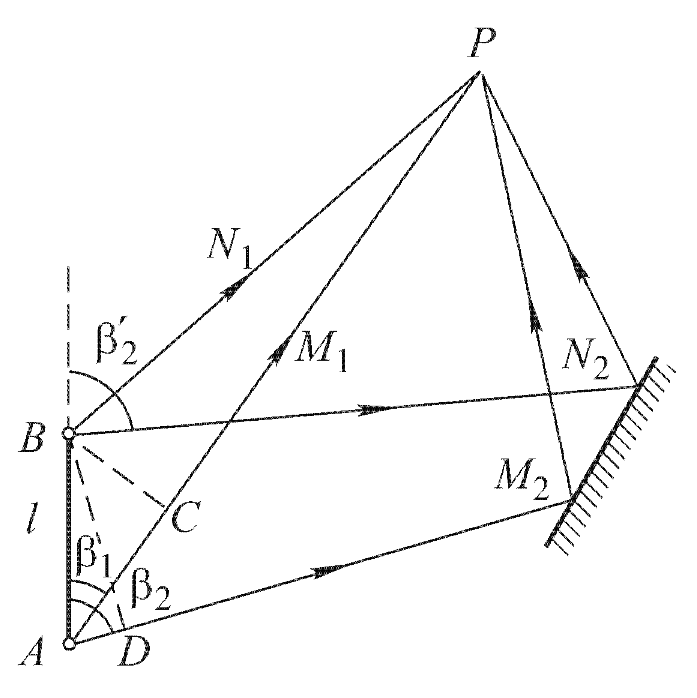
\includegraphics[width=0.3\textwidth]{figures/28_1.png}
    \hspace{5 mm} 
    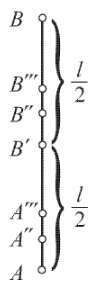
\includegraphics[width=0.09\textwidth]{figures/28_2.png}
    \caption{К пространственной когерентности}
    \label{fig281}
\end{figure}
Считая $l=AB$ достаточно малым, то для разности оптических лучей можно написать $l\cos \beta_1$ и $l \cos \beta_2$. Тогда для разности оптической разности хода лучей от $A$ и $B$ верно, что
\begin{equation*}
    \Delta = 
    \left[(AM_1P)-(AM_2P)\right]-\left[(BN_1 P) - (BN_2P)\right]
   = l |\cos \beta_1 - \cos \beta_2|,
\end{equation*}
которая определяет сдвиг одной интерфереционной картины относительно другой. При $\Delta = \lambda/2$ максимумы одной -- минимумы другой, при $\Delta = \lambda$ резонируют. 

Стоит заметить, что мы условно считаем, что при $\Delta = (m+1/4)\lambda,\, m \in \mathbb{Z}$ -- всё хорошо. А ещё $\beta = \beta'$. 



\textbf{Протяженный источник}.  Считая, что все точки излучают некогерентно, разобьём на пары источников $(A, B'),\,  (A'', B'')$ и т.д. находящиъся на $l/2$ друг от друга. Тогда, при $\Delta/2 = \lambda/2$ от каждой пары будет просто светлый фон, получаем условия
\begin{equation*}
    \Delta \equiv l(\cos \beta_2 - \cos \beta_2) = m\lambda,
\end{equation*}
при выполнении которого на экране один только освещенный фон без полос. При $\Delta = (m+\alpha)\lambda$ источник можно разбить на две части $m \colon  \alpha$, где меньшая часть источника даст интерференционные полосы на светлом фоне от большей части источника. 

Если крайние лучи выходят симметрично к $\bot AB$, т.е. $\beta_2 = \pi-\beta_1$, то $\cos \beta_2 = - \cos \beta_1$, и тогда хорошая интерференция будет при
\begin{equation*}
    (l/2) |\cos\beta_1-\cos \beta_2| \leq \lambda/4,
    \hspace{10 mm} 
    l \sin (\Omega/2) \leq \lambda/4,
\end{equation*}
где $\Omega$ -- угол между крайними лучами, угол интерференциии. 


\begin{to_def}
    Два источника, позволяющие наблюдать интереференцию света от них, называют \textit{пространственно когерентными}, иначе -- \textit{пространственно некогерентными}. 
\end{to_def}

В случае же монохроматичного света, можем говорить про пространственную когерентность при 
\begin{equation*}
    \sigma =\pi \lambda^2 / (4 \varphi^2). 
\end{equation*}

\Ssec{32}{Теорема Ван-Циттера-Цернике}
\subsection{Теорема Ван-Циттера-Цернике}

Пространственную когерентность $\gamma_{1, 2}$ для точек $Q_1$ и $Q_2$ экрана, освещаемого протяженным квазимонохроматическим самосветящимся источником света. Если рассматриваемая точка $P$ равноудалена от $Q_1$ и $Q_2$ то можем рассматривать просто волны в $Q_1$ и $Q_2$. В качетсве источника рассматривается площадка $\sigma$ $\parallel$ экрану. 


В точках $Q_1$ и $Q_2$ может быть определена интенсивность
\begin{equation*}
    I_1 \equiv I(Q_1) = \int_\sigma \frac{I(S) \d S}{r_1^2}, \hspace{5 mm} 
    I_2 \equiv I(Q_2) = \int_\sigma \frac{I(S) \d S}{r_2^2}.
\end{equation*}
Введя нормирующий множитель, можем найти $\gamma_{1,2} (\theta \ll 1)$:
\begin{equation*}
    \gamma_{1,2} (0) = \frac{1}{\sqrt{I_1 I_2}} \int \frac{I(S)}{r_1 r_2} e^{ik (r_2-r_1)} \d S.
\end{equation*}
Таким образом мы говорим, что:

\begin{to_thr}[теорема Ван-Циттера-Цернике]
    Комплексная степень взаимной когерентности в точках $Q_1$ и $Q_2$ равна комплексной амплитуде в точке $Q_1$ соответстствующей дифрагированной волны.
\end{to_thr}


\Qsec{16}{Дифракция в оптических приборах}

\Ssec{56}{Разрешающая способность при когерентном и некогерентном освещении}
Рассматриваем идеальные оптические системы, а конечный рассматриваемый объект как совокупность точечных источников, каждый из которых изображается кружком Эйри(с окружающими его дифракционными кольцами).
Наша задача сводится к рассмотрению двух случаев точечных
\begin{enumerate}
	\item некогерентных источников --- складываются их интенсивности --- самосветящиеся --- телескоп;
	\item когерентых источнико --- складываются их напряженности --- освещаемые --- микроскоп.
\end{enumerate}

Разрешающие способности соответственно:
\begin{equation*}
	\text{телескоп: } \vartheta_\text{мин} = 1,22 \frac{\lambda}{D}
	\hspace{2 cm}
	\text{микроскоп: } l_\text{мин} = 0.61 \frac{\lambda}{n \sin \alpha} 
\end{equation*}
где $\alpha$ -- апертурный угол, $l$ -- расстояние между кружками Эйри, $\vartheta$ -- угловой размер наблюдаемого объекта.

\Qsec{17}{Дифрационная решетка}

\Ssec{46}{Дифракционная решетка}

\begin{minipage}{0.45\textwidth}
    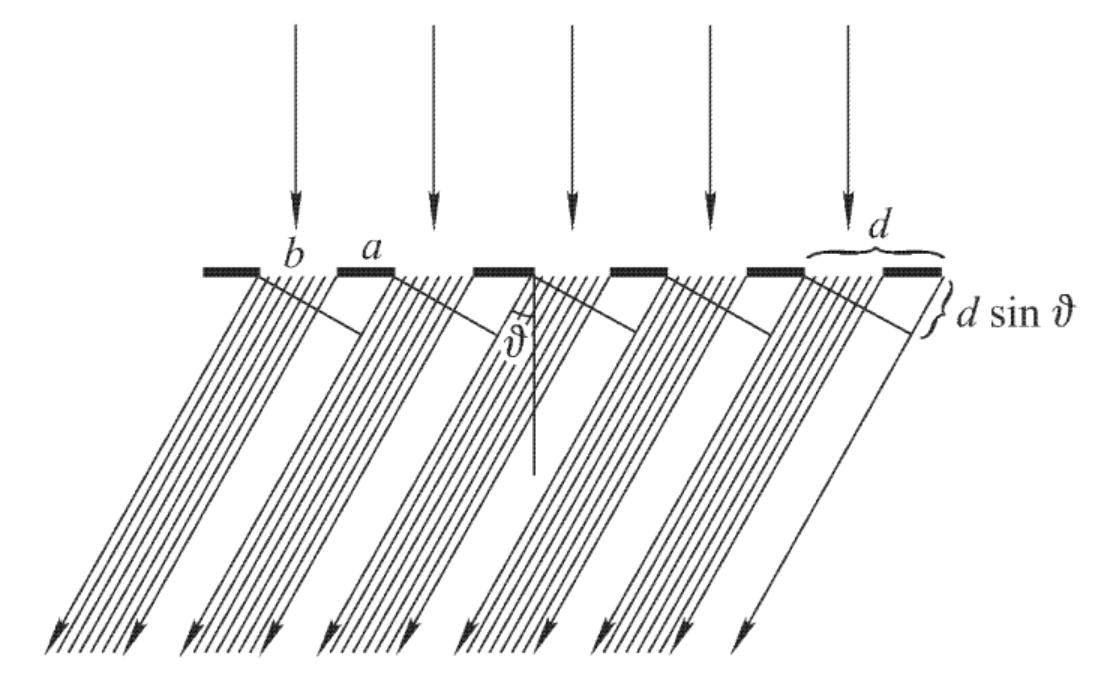
\includegraphics[width=1\textwidth]{figures/s36_1.png}
\end{minipage}
\hfill
\begin{minipage}{0.45\textwidth}
	Имеем простейший случай: лучи падают перпендикулярно, $d$ -- \textit{период решетки}, $\vartheta$ -- угол дифракции.
	Разность хода между волнами, исходящими из соседних щелей 
	\begin{equation*}
		\Delta = d \sin \vartheta, 	
	\end{equation*}
	а разность фаз 
	\begin{equation*}
		\delta = k d \sin \vartheta = 2 \pi d \sin \vartheta / \lambda.
	\end{equation*}  
	Поле, наблюдаемое от первой щели определяется формулой
	\begin{equation*}
		E_1 = \frac{b \sin\alpha}{\alpha}.
	\end{equation*}
\end{minipage}

Поля же излучаемые остальными щелями:
\begin{equation*}
	E_2 = E_1 e^{-i \delta}, 
	\hspace{0.5 cm}
	E_3 = E_1 e^{-2i \delta},
	\hspace{0.5 cm}
	\ldots
	\hspace{0.5 cm}
	E_N = E_1 e^{- i (N-1)\delta}.
\end{equation*}
Полное поле представится как сумма всех:
\begin{equation*}
	E = E_1 \frac{1- e^{- i N \delta}}{1 - e^{-i\delta}} = E_1 \frac{\sin \left(\frac{N \delta}{2}\right)}{\sin \left(\frac{\delta}{2}\right)}e^{- i (N-1)\delta/2}
	\hspace{1 cm}
	\Rightarrow
	\hspace{1 cm}
	I = I_1 \left[\frac{\sin \left(\frac{N \delta}{2}\right)}{\sin \left(\frac{\delta}{2}\right)}\right]^2.
\end{equation*}
Заметим, что при  
\begin{equation*}
	\delta/2 = m \pi
	\hspace{1 cm}
	\Leftrightarrow
	\hspace{1 cm}
	d \sin \vartheta = m \lambda.
\end{equation*}
получаем $I = N^2 I_1$ -- \textit{главные максимумы}, где $m$ -- целое число, \textit{порядок главного максимума}. Это соотношение так же определяет направление $\vartheta$ на главные максимумы.

Если у решетки $a = b$, то все главные максимумы четных порядков вообще не появятся, так как условие максимума решетки перейдёт в условие минимума дифракции на одной щели $I_1=0$:
\begin{equation*}
	d \sin \vartheta = 2 n \lambda
	\hspace{1 cm}
	\Rightarrow
	\hspace{1 cm}
	b \sin \vartheta = n \lambda.
\end{equation*}
Таким образом в рассматриваемом направлении ни одна щель, а потому и решетка в целом не излучают.

Дифракционные минимумы получаются из условия:
\begin{equation*}
	d \sin \vartheta = \left(m \frac{p}{N}\right)\lambda.
\end{equation*}
Максимумы, получающиеся между двумя соседними минимумами, называются \textit{второстепенными максимумами}. 
Таким образом между двумя соседними максимумами располагается $(N-1)$ минимум и $(N-2)$ добавочный максимум. И на эту всю красоту накладывается минимумы дифракции на одной щели.

Второстепенные максимумы находятся примерно между минимумами давайте определим направление $\delta$ на них:
\begin{equation*}
	\frac{\delta}{2} = \left(m + \frac{2 p +1}{2 N}\right)\pi.
\end{equation*}

Найдём теперь интенсивность второстепенных максимумов в окрестности главного, то есть при $N \gg 1$ и малых номерах этих максимумов $p$, а $\delta/2$ -- мал:
\begin{equation*}
	\sin \frac{\delta}{2} = \pm \sin \frac{2 p +1}{2 N} \approx \pm \frac{2 p +1}{2 N} \pi
	\hspace{0.5 cm}
	\Rightarrow
	\hspace{0.5 cm}
	I = \frac{I_1}{\pi^2}\left(\frac{2N}{2p+1}\right)^2 = \frac{4}{(2p +1)^2 \pi^2}I_\text{гл}.
\end{equation*}
Таким образом интенсивности максимумов к главному относятся как очень малые величины. И при большом числе щелей они вообще не играют роли.

\begin{minipage}{0.35\textwidth}
    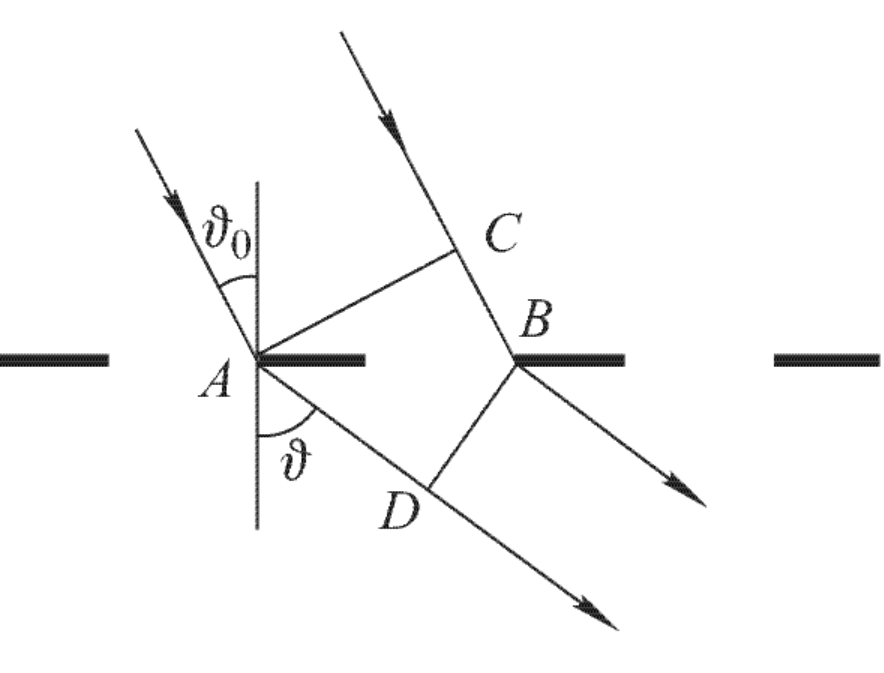
\includegraphics[width=1\textwidth]{figures/s46_2.png}
\end{minipage}
\hfill
\begin{minipage}{0.55\textwidth}
	Если же волна падает на решетку под углом, то разность хода между соседними щелями становится равной:
	\begin{equation*}
		d (\sin \vartheta - \sin \vartheta_0).
	\end{equation*}
	Мы имеем новое условие на главные максимумы:
	\begin{equation*}
		d (\sin \vartheta - \sin \vartheta_0) = m \lambda,
	\end{equation*}
	а минимумы:
	\begin{equation*}
		d(\sin \vartheta - \sin \vartheta_0) = \left(m + \frac{p}{N}\right) \lambda.
	\end{equation*}
\end{minipage}

И наконец если решетка -- грубая, то при углах падения $\vartheta_0$ близких к $90^\circ$ можно написать:
\begin{equation*}
	d \cos \vartheta_0 \cdot (\vartheta - \vartheta_0) = m \lambda.
\end{equation*}
Где $d \cos \vartheta_0$ -- типа новый период, который мы уже вправе от угла падения уменьшать, делая решетку менее грубой.

\Qsec{18}{Спектральные приборы}

\Ssec{48}{Эшелон Майкельсона и интерференционные спектральные приборы}

\begin{figure}[h]
    \centering
    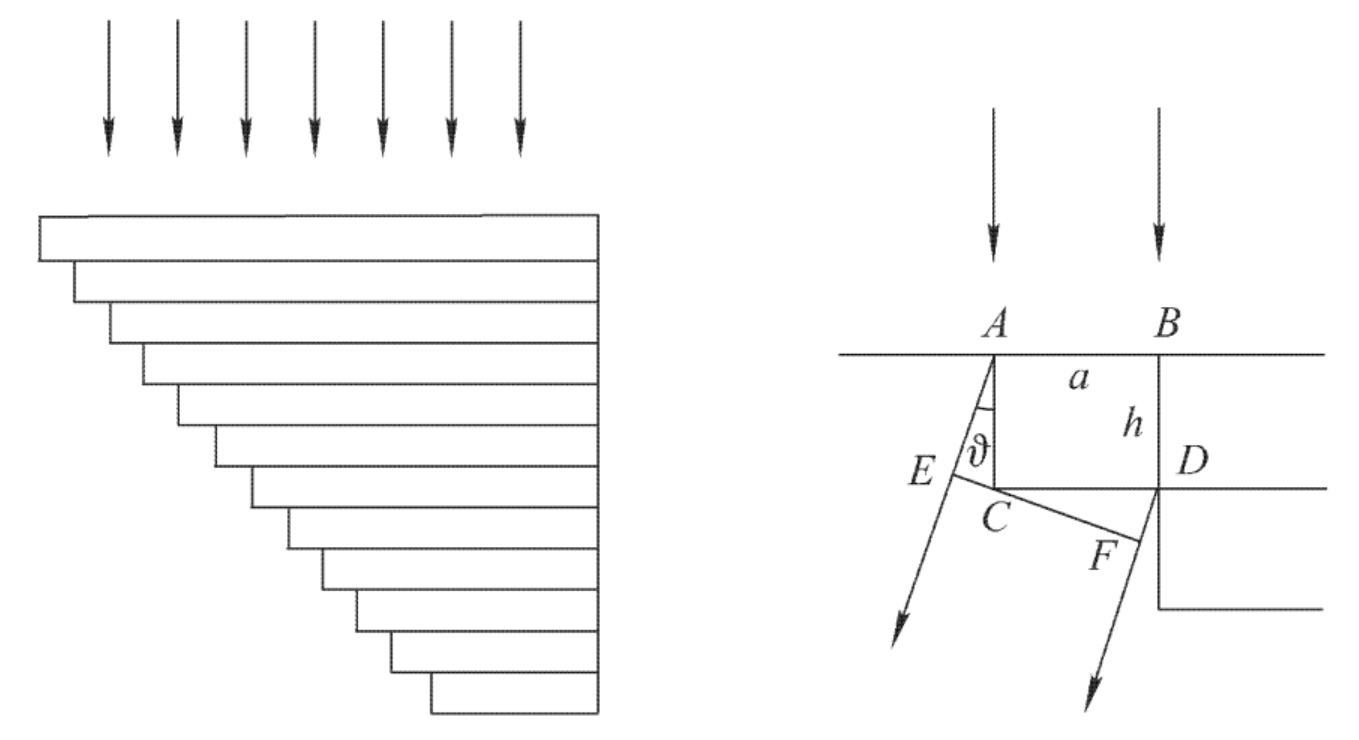
\includegraphics[width=0.45\textwidth]{figures/s47_1.png}
    %\caption{}
    %\label{fig:}
\end{figure}
Для такой картинки разность хода будет:
\begin{equation*}
	\Delta = n h + a \sin \vartheta - h \cos \vartheta = m \lambda.
\end{equation*}
Положения главных максимумов определятся из условия
\begin{equation*}
	nh + a \sin \vartheta - h \cos \vartheta = m \lambda.
\end{equation*}
Найдём дисперсию:
\begin{equation*}
	\frac{d \vartheta}{d \lambda} = \frac{m}{a \cos \vartheta + h \sin \vartheta} \approx = \frac{a}{m} = \frac{h (n-1)}{a \lambda}.
\end{equation*}
Что описывает эшелона как достаточно хороший спектрометр. Его дисперсионная область:
\begin{equation*}
	\Delta \lambda = \frac{\lambda}{m} = \frac{\lambda^2}{h (n-1)}.
\end{equation*}
Она очень мала, что является большим недостатком эшелона.

Разрешающая способность: 
\begin{equation*}
	R = \frac{\lambda}{\delta\lambda} = N m = \frac{N h (n-1)}{\lambda}.
\end{equation*}
Эту формулу можно уточнить, приняв во внимание дисперсию по длине волны от стекла:
\begin{equation*}
	\frac{\lambda}{\delta\lambda} = \frac{N h}{\lambda} \left[(n-1) - \lambda \frac{d n}{d \lambda}\right].
\end{equation*}
И аналогичные аналогичными рассуждениями:
\begin{equation*}
	\Delta\lambda = \frac{\lambda}{m - h (d n / d\lambda)},
	\hspace{0.5 cm}
	\frac{d \vartheta}{d \lambda} = \frac{m - h (d n/d \lambda)}{a \cos \vartheta + h \sin \vartheta}.
\end{equation*}	

\Ssec{49}{Разрешающая способность призмы}


Пусть на призму падает $\lambda'$. Будем рассматривать симметричный ход лучей (рис. \ref{fig:pr}). 
\begin{figure}[h]
    \centering
    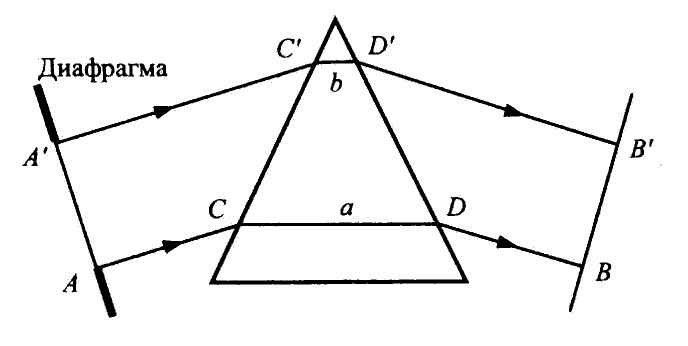
\includegraphics[width=0.4\textwidth]{figures/49_1.png}
    \caption{Призма, как спектральный прибор}
    \label{fig:pr}
\end{figure}
Начальное положение волнового $AA'$, а после $BB'$. Поскольку $BB'$ -- это участок волнового фронта, то данное направление можно рассматривать как направление на дифракционный максимум $m=0$ для $\lambda'$. 

По критерию Рэлея направление на дифракционный минимум $\lambda$ должен совпадать с максимумом $\lambda'$, тогда разность хода лучей $AB$ и $A' B'$ равна длине волны:
\begin{align*}
    &\text{max:} \ \ 
    &\left[AC + n(\lambda') a + DB\right] - \left[
        A'C' + n(\lambda') b + D' B'
    \right] = 0, \\
    &\text{min:} \ \ 
    &\left[AC + n(\lambda) a + DB\right] - 
    \left[
        A'C' + n(\lambda) b + D' B'
    \right] = \lambda,
\end{align*}
где $AA'$ и $BB'$ уже не представляют участков волнового фронта.  Вычитая два последних равенства, находим
\begin{equation*}
    \left[n(\lambda)-n(\lambda')\right]a - \left[n(\lambda)-n(\lambda')\right]b = \lambda,
\end{equation*}
что при рассмотрении близких $\lambda' - \lambda \ll\lambda$ и считая $\Delta \lambda = \lambda'-\lambda$ перейдёт в 
\begin{equation*}
    -(a-b) \frac{d n}{d \lambda} \Delta \lambda = \lambda,
    \hspace{0.5cm} \Rightarrow \hspace{0.5cm}
    R = \frac{\lambda}{\Delta \lambda} = - (a-b) \frac{d n}{d \lambda},
\end{equation*}
где $R > 0$ при $n'_\lambda < 0$ в области нормальной дисперсии.

\Qsec{19}{Дифракционная решетка как спектральный прибор}


\Ssec{47}{Дифракционная решетка как спектральный прибор}

Как мы видели выше дифракционная решетка имеет раскидывать волны, падающие на нее, под разными углами. Введём характеристики такого спектрального прибора.

\textbf{Угловой дисперсией} называют производную $d \vartheta/ d \lambda$. Чем она больше, тем больше расстояние между двумя спектральными линиями.
\begin{equation*}
	\frac{d}{d \lambda} \big[ d (\sin \vartheta - \sin \vartheta_0) = m \lambda \big]
	\hspace{1 cm}
	\leadsto
	\hspace{1 cm}
	\frac{d \vartheta}{d \lambda} = \frac{m}{d \cos \vartheta} = \frac{\sin \vartheta  - \sin \vartheta_0}{\lambda \cos \vartheta}.
\end{equation*}
Таким образом угловая дисперсия не зависит от параметров решетки, а определяется только длинами волн и углами падения и дифракции.

\textbf{Дисперсионная область} -- максимальная ширина спектрального интервала $\Delta \lambda$, при котором ещё нет перекрытия спектральных линий.

Пусть падающие длины лежат в диапазоне: $\lambda' = \lambda + \Delta \lambda$. Пусть $(m+1)$ порядок $\lambda$ с $m$ порядком  $\lambda'$.
Тогда
\begin{equation*}
	\left\{
	\begin{aligned}
		&d (\sin \vartheta - \sin \vartheta_0) = m \lambda'\\
		&d (\sin \vartheta - \sin \vartheta_0) = (m+1) \lambda	
	\end{aligned}
	\right.
	\hspace{0.5 cm}
	\Rightarrow
	\hspace{0.5 cm}
	m \lambda' = (m+1) \lambda
	\hspace{0.5 cm}
	\Rightarrow
	\hspace{0.5 cm}
	\lambda' - \lambda \equiv \Delta \lambda = \lambda/m.
\end{equation*}

\textbf{Разрешающая способность} аппарата -- $R = \frac{\lambda}{\delta \lambda}$. А наименьшая разность длин волн двух спектральных линий $\delta\lambda$, при которой спектральный аппарат разрешает эти линии, называется \textit{спектральным разрешаемым расстоянием}.
То есть мы стремимся, чтобы дифракционные картины около каждого спектра были как можно более узкими, вдобавок к узкой дисперсии.

Спектральные линии с близкими длинами волн $\lambda$ и $\lambda'$ считаются разрешенными, если главный максимум дифракционной 
картины для одной длины волны совпадает по своему положению с первым дифракционным минимумом в том же порядке для другой длины волны. 
\begin{equation*}
	\left\{
	\begin{aligned}
		&d (\sin \vartheta - \sin \vartheta_0) =  m \lambda'\\
		&d (\sin \vartheta - \sin \vartheta_0) = \left(m+\frac{1}{N}\right) \lambda	
	\end{aligned}
	\right.
	\hspace{0.5 cm}
	\Rightarrow
	\hspace{0.5 cm}
	m \lambda' = (m+\frac{1}{N}) \lambda
	\hspace{0.5 cm}
	\Rightarrow
	\hspace{0.5 cm}
	\lambda' - \lambda \equiv \delta \lambda = \lambda/(N ms).
\end{equation*}
Таким образом получаем критерий Релея $R = \frac{\lambda}{\delta\lambda} = N m$.

\Qsec{20}{Интерферометр Фабри-Перо}


\Ssec{36}{Многолучевая интерференция}



\textbf{Прошедшая волна}.
Обозначим через $R$ коэффицент отражение света от границы раздела пластинки с воздухом. При отсутсвии поглощения $(1-R)$ проходит через границу, если среды по обе стороны одинаковы, то и $R$ будут одинаковы. Пусть свет монохроматичен
Пусть интенсивность света $I_0$, тогда интенсивности прошедших пучков будут
\begin{equation*}
    I_{1'} = (1-R)^2, \hspace{5 mm} 
    I_{2'} = R^2(1-R)^2 I_0, \hspace{5 mm} 
    I_{3'} = R^4 (1-R)^2 I_0, \hspace{5 mm}  \ldots
\end{equation*}
а соответсвеющие вещественные амплитуды
\begin{equation*}
    a_{1'} = (1-R) a_0, \hspace{5 mm} 
    a_{2'} = R(1-R) a_0, \hspace{5 mm} 
    a_{3'} = R^2(1-R) a_0, \ldots .
\end{equation*}
Амплитула прошедшей волны представится убывающей геометрической прогрессией
\begin{equation*}
    \sub{a}{d} = a_0 (1-R)\left[1 + R e^{-i \Phi} + R^2 e^{-2i \Phi} + \ldots\right],
    \hspace{5 mm} 
    \Phi = k \Delta = \frac{4 \pi}{\lambda} n d \cos \psi,
    \hspace{0.5cm} \Rightarrow \hspace{0.5cm}
    \sub{a}{d} = \frac{1-R}{1-R e^{-i\Phi}} a_0.
\end{equation*}
где $\Phi$ -- разность фаз между соседними пучками.  Интенсивность прошедшей волны
\begin{equation*}
    \sub{I}{d} = \frac{(1-R)^2}{|1-R e^{-i \Phi}|^2} a_0^2 = \frac{(1-R)^2}{(1-R)^2 + 4 R \sin^2 (\Phi/2)} I_0,
\end{equation*}
что позволяет сделать некоторые выводы. 



\textbf{Отраженная волна}. Аналогичный расчёт приведет к
\begin{align*}
    &I_1 = R I_0, 
    &I_2 = R(1-R)^2 I_0, 
    &&I_3 = R^3 (1-R)^2 I_0, 
    &&\ldots, \\ 
    &a_1 = \sqrt{R} a_0, 
    &a_2 = - \sqrt{R} (1-R) a_0, 
    &&a_3 = - \sqrt{R} R (1-R) a_0, 
    &&\ldots,
\end{align*}
где знак в $a$ -- следставие появления $\lambda/2$. Резуьтирующая амплитуда будет иметь вид
\begin{equation*}
    a_r = \sqrt{R} a_0 - \sqrt{R} (1-R) a_0 e^{-i \Phi} \left[
        1 + R e^{- i \Phi} + R^2 e^{-2i \Phi} + \ldots
    \right],
    \hspace{0.5cm} \Rightarrow \hspace{0.5cm}
    I_r = \frac{4 R \sin^2 (\Phi/2)}{(1-R)^2 + 4 R \sin^2(\Phi/2)} I_0, 
\end{equation*}
где всё также $\Phi = k \Delta = \frac{4 \pi}{\lambda} n d \cos \psi$.


При $R \ll 1$ увидим случай двулучевой интерференции, при $R \approx 1$ уже интереснее (рис. \ref{fig:piks}). 
\begin{figure}[ht]
    \centering
    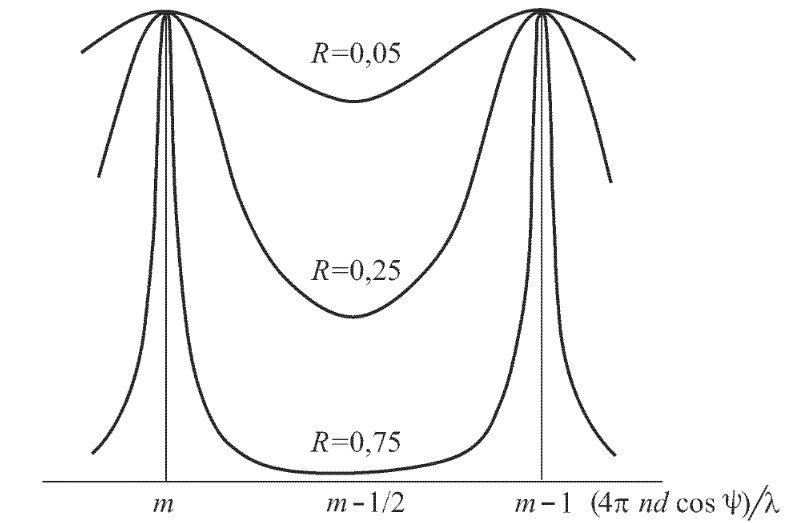
\includegraphics[width=0.3\textwidth]{figures/36_1.png}
    \caption{Пики для пластинки}
    \label{fig:piks}
\end{figure}
В окрестности максимума $m$-го порядка $\Phi = \pi m + \varphi$, тогда ввиду малости $\varphi$ можем написать
\begin{equation*}
    \sub{I}{d} = \frac{I_{\text{max}}}{1 + R \varphi^2/(1-R^2)},
    \hspace{0.5cm}
    \frac{R \varphi^2}{(1-R)^2} = 1 \text{ при } \sub{I}{d}= \frc{1}{2} \sub{I}{max},
    \hspace{0.5cm} \Rightarrow \hspace{0.5cm}
    \Delta \Phi = 2 \varphi = 2 \frac{1-R}{\sqrt{R}}.
\end{equation*}




\Esec{Интерферометр Фабри-Пера}
\textbf{Разрешающая способность}. Имеем дело с интерференцией высоких порядков, поэтому требуется высокая \textit{монохроматичность света} ($\lambda/\delta \lambda \gg m$).

\begin{to_def}
    Разрешающая способность определяет наименьшее расстояние между близкими спектральными линиями, которые изображаются в виде раздельных спектральных линий. Если максимум одного пика находится не ближи полуширины другого, то их считают различимыми. 
\end{to_def}


Определим минимальную разность $\delta \lambda = \lambda'-\lambda$. Для интерферометра Фабри-Перо верно, что $n$ одинаков для двух длин волн. В точке $A'$ -- максимум $m$-го порядка для $\lambda'$, а потому $\Phi' = 2 \pi m$. В той же точке $\lambda$ имеет разность фаз $\Phi = 2 \pi m + (1-R)/\sqrt{R}$, т.е в рассматриваемой точке $\Phi'-\Phi = \delta \Phi = (1-R)/\sqrt{R}$. Но ввиду $n = n'$ верно, что $\delta \Phi / \Phi = |\delta \lambda / \lambda|$. Учтя, что в максимуме $\Phi = 2 \pi m$, находим
\begin{equation*}
    \frac{\lambda}{\delta \lambda} = \frac{2 \pi \sqrt{R}}{1-R} m, \text{ --- \textit{разрешающая способность спектрального прибора}.}
\end{equation*}


Он состоит из двух стеклянных 
или кварцевых пластинок $P_1$ и $P_2$, между которыми обычно находится воздух. Отражающая способность доводится до 95-98 \%, шероховатости допустимы в пределах $0.01 \lambda$. 
\begin{figure}[ht]
    \centering
    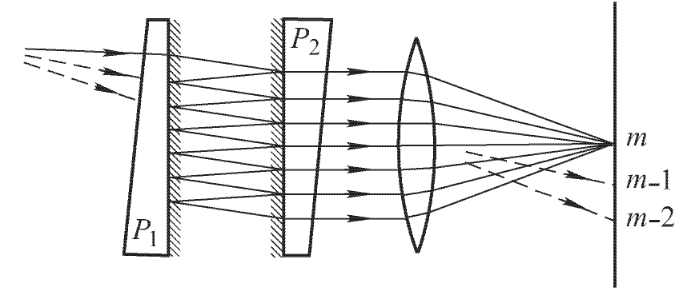
\includegraphics[width=0.5\textwidth]{figures/36_2.png}
    \caption{Интерферометр Фабри-Перо.}
    \label{fig:fp}
\end{figure}
Интерференционная картина состоит из концентрических колец равного наклона. Ввиду малости угла $\psi$ условие главного интерференционного максимума $2 h \cos \psi = m \lambda$ можно записать в виде $h(2-\psi^2) = m\lambda$ откуда \textit{угловая дисперсия} равна
\begin{equation*}
    \frac{d \psi}{d \lambda} = - \frac{m}{2 h \psi} = - \frac{1}{\lambda \psi},
\end{equation*}
которая значительно превышает дисперсию других спектральных приборов. 



\textbf{Интерферометр Фабри-Перо как резонатор}.
В этом разделе волны распространяются нормально к поверхности резонатора. Соответсвенно прибор прозрачен для длин вол излучения, удовлетворяющих условию $m \lambda = 2 L \cos \theta = 2 L$. Также $L$ -- расстояние между зеркалами $\gg \lambda$, а также $1-R \ll 1$. Добротность запишем, как
\begin{equation*}
    Q = 2 \pi \frac{E_0}{\Delta E}, 
\end{equation*}
где $E_0$ -- накопленная энергия, а $\Delta E$ -- энергия, теряемая за период колебаний. 
В указанных предположениях верно, что есть стоячая волна, эквивалентная суперпозиции двух бегущих. 



\begin{to_def}
    \textit{Резонатор} -- колебательная система, устройство, способное накапливать энергию колебаний, поставляемую из внешнего источника. 
\end{to_def}


Если поток энергии в каждой их волн равен $P$, то энергия равна 
\begin{equation*}
    E_0 = 2 P \tau_L = 2 P L/c,
\end{equation*}
где $\tau_L = L/c$ -- время, за которое волна проходит расстояние $L$ между пластинами. Поскольку можность потерь составляет $(1-R) 2 P$, то за период колебаний $T$ теряется энергия 
\begin{equation*}
    \Delta E = 2 P (1-R) T.
\end{equation*}
Так как $\lambda = c T$, то по определению находим
\begin{equation*}
    Q = 2 \pi \frac{E_0}{\Delta E_0} = 2 \pi \frac{L}{\lambda} \frac{1}{1-R}.
\end{equation*}
Зная добротность, мы можем найти эффективную ширину линии излучения, выходящего из резонатора:
$\Delta \sub{\lambda}{eff} = \lambda/Q$, по определению добротности $Q = \omega / \Delta \omega$, преобразованного с помощью равенства $\Delta \omega/\omega = \Delta \lambda/\lambda$ вытекающего из $\omega = 2 \pi c / \lambda$. В таком случае приходим к формуле вида
\begin{equation*}
    \Delta \lambda = \lambda \frac{\Delta \nu}{\nu} = \frac{\lambda^2}{2L}.
\end{equation*}
Таким образом выделяемые резонатором линии являются в высокой степени монохроматическими. 

Теперь читателю предоставляется прочитать текст идущий далее, а потом вернуться к этим строчкам, где я опишу интерферометр Фабри-Перо как спектральный прибор.
Если он у нас заполнен однородной однородной средой с показателем преломления $n$. 

Порядок спектра $m = 2 h/\lambda$, где $h$ -- расстояник между отражающими поверхностями. Для такого порядка спектра:
\begin{equation*}
    \delta\Phi = (1-R)/\sqrt{R},
    \hspace{0.5 cm}
    \Phi_{\text{max}} = 2 \pi m,
    \hspace{0.5 cm}
    \Phi_{\text{min}} = \frac{4 \pi d n \cos \psi}{\lambda}.
\end{equation*}
Только теперь $n$ и $\psi$ имеют разные значения для $\lambda$ и $\lambda'$. И только $n\sin \psi = n' \sin \psi' = \sin \varphi$. Тогда должно быть:
\begin{equation*}
    \frac{\delta \Phi}{\Phi} = \frac{\delta n}{n} - \frac{\sin \psi \delta \psi}{\cos \psi}- \frac{\delta \lambda}{\lambda}.
\end{equation*}
С помощью условия:
\begin{equation*}
    \frac{\delta n}{n} + \frac{\cos \psi}{\sin \psi} \delta \psi = 0
    \hspace{1 cm}
    \Rightarrow
    \hspace{1 cm}
    \frac{\delta \Phi}{\Phi} = \frac{1}{\cos^2 \psi}\frac{\delta n}{n} - \frac{\delta \lambda}{\lambda}.
\end{equation*}
То, подставляя значения $\delta \Phi$, $\Phi_{\text{max}}$ и $\delta n = \left(\frac{d n}{d \lambda}\right) \delta \lambda$ \textit{разрешающая способность} получается
\begin{equation*}
    R = \frac{\lambda}{\delta\lambda} = \frac{2 \pi \sqrt{R} m}{1 - R}\left(1 - \frac{1}{\cos^2 \psi} \frac{\lambda}{n} \frac{d n}{d \lambda}\right).
\end{equation*}




\Qsec{21}{Принципы фурье-оптики}


\Ssec{52}{Дифракция на решетке как краевая задача}
\subsection{Дифракция на решетке как краевая задача}

\subsubsection{Метод Рэлея}
Пусть решетка -- бесконечна, её переднюю поверхность будем называть \textbf{входом}, а заднюю -- \textbf{выходом}. Плоскость решетки примем за $XY$, а ось $Z$ по распространению волны.

Падающую волну представим в виде: $E_0 = A e^{i (\omega t - \smallvc{k} \smallvc{r})}$.
Тут полагаем $z = 0$, ищем поле на входе решетки, в силу линейности $E_{\text{вых}} = D E_{\text{вх}}$.

Здесь введен коэффициент пропускания $D$ решетки. 
Теперь чтобы решить задачу о дифракции на решетки нам достаточно найти $D$, тогда мы уже будем знать поле на выходе из решетки, а значит и во всем пространстве дальше. Уравнение
\begin{equation*}
	\Delta E + k^2 E = 0
\end{equation*}
должно при $z = 0$ переходить в $E_{\text{вых}}(x,y) = D(x,y) E_{\text{вх}}(x,y)$. Такой подход к решению задача называется \textit{методом Рэлея}.

Для одномерной решетки можно представить $D$ как функцию с периодом $d$:
\begin{equation*}
	D = \sum_{m =- \infty}^{+\infty}D_m e^{-i m p x},
	\hspace{0.5 cm}
	p =\frac{2 \pi}{d}.
\end{equation*}
Таким образом:
\begin{equation*}
	E_\text{вых} = D E_\text{вх} = \sum_{m = - \infty}^{+\infty} A D_m e^{i [\omega t - (k_x + m p)x]}.
\end{equation*}
Общим решением нашего волнового уравнения будет:
\begin{equation*}
	E = \sum_{m = - \infty}^{+\infty} a_m e^{i(\omega t - \smallvc{q_m} \vc{r})},
\end{equation*}
на которое надо наложить в связи с граничным условием:
\begin{equation*}
	q_{mx} = k_x + m p, \hspace{0.5 cm} q_{m y} = 0.
\end{equation*}
И так как $\vc{q}^2 - k^2$, то $q_{mz} = \sqrt{k^2 - q_{mx}^2}$ -- для однородных волн и $q_{mz} = -i \sqrt{k^2 - q_{mx}^2}$ для неоднородных (поверхностных).

Тогда для поля на выходе можно написать:
\begin{equation*}
	E_\text{вых} = \sum_{-\infty}^{+\infty} a_m e^{i (\omega t - q_{mx} x)}
	\hspace{0.5 cm}
	\Rightarrow
	\hspace{0.5 cm}
	a_m = A D_m.
\end{equation*}

Теперь если $k_x = \left(\frac{2\pi}{\lambda}\right)\sin \theta$, $q_{mx} = \left(\frac{2\pi}{\lambda}\right) \sin\vartheta_m$ и $p = 2\pi/d$ то получаем основную формулу дифракционной решетки:
\begin{equation*}
	d (\sin \vartheta_m - \sin \theta) = m \lambda.
\end{equation*}
Что видим? Спектр за решеткой состоит из одних только главных максимумов, но это нормально, так как решетка бесконечна. 
В формулу для волны входят как однородные так и не однородные волны, а значит она описывает поле на любых расстояниях от решетки.
При нормальном падении света наивысший порядок однородных волн $m\leq d/\lambda$, иначе имеем неоднородные волны, которые затухают как $\exp(-\chi_m z)$, где
\begin{equation*}
	\chi_m = \sqrt{k^2 - q_{mz}^2} = \frac{2 \pi}{d} \sqrt{m^2 - (d/\lambda)^2}.
\end{equation*}

Интересно по-исследовать поле далеко от решетки. При $z \gg d$ оно состоит только из однородных волн. А если $d<\lambda$ то вообще из одной плоской волны ($m = 0$). 

Тут можно найти красивый эффект \textbf{саморепродукции}. 
Каждое слагаемое в разложении нашей волны -- поле плоской волны с пространственной частотой: $u_n = n \frac{2 \pi}{d}$. Для точки отстоящей на $z$ от решетки фаза $n$-ой плоской волны:
\begin{equation*}
	\varphi_n = \chi_n z = \sqrt{k^2 - q_{nx}^2} \approx k z - \frac{z q_{nx}^2}{2 k},
\end{equation*}
что верно для волн с узким спектром $|q|\ll k$.

Сравним набег фаз $n$-ой плоской волны с $\varphi_0 = kz$:
\begin{equation*}
	\Delta \varphi_n = \varphi_0 - \varphi_n = \frac{z}{2k}\left(\frac{2 \pi}{d}\right)^2 n^2 = \pi \frac{\lambda z}{d^2}n^2.
\end{equation*}
В плоскости наблюдения отстоящую от решетки на $z_1 = \frac{2 d^2}{\lambda}$ (это будет находится в зоне френелевской дифракции) будем иметь разность фаз $\Delta \varphi_n = 2 \pi n^2$. Заметим так же, что разность фаз от любых двух плоских волн будет $\Delta \varphi = 2 \pi (n_1^2 - n_2^2)$ тоже кратна $2\pi$. 
Значит в разложении волны ничего не меняется, так как это период, значит в плоскости $z_1$ поле повторяет по интенсивности пропускающую функцию решетки, ну а точнее:
\begin{equation*}
	f(x,z_1) = e^{i k z_1}f_0(x).
\end{equation*}
Это же свойство повторения характерно и для
\begin{equation*}
	z_m = m \frac{2 d^2}{\lambda} \, (m = 1,2 \ldots).
\end{equation*}
Этот эффект еще также носит названия \textbf{эффекта Таблота}.


Теперь посмотрим на небесконечную решетку.
\begin{equation*}
	D(x) = \int_{-\infty}^{+\infty} C(f) e^{-i f x} d f.
\end{equation*}
На выходе поле:
\begin{equation*}
	E_\text{вых} = A \int_{-\infty}^{+\infty} C(f) e^{-f(k_x +f)x}d f.
\end{equation*}
Решение тогда будет:
\begin{equation*}
	E = A \int_{-\infty}^{+\infty} C(f) e^{- i \smallvc{q} \smallvc{r}} d f.
\end{equation*}
Задавая функцию пропускания для такой конечной решетки:
\begin{equation*}
	D(x) =\left\{
	\begin{aligned}
		0, \text{ если } -\infty < x < - L,\\
		\sum_{-\infty}^{_\infty} D_m e^{i m p x}\text{ если } - L < x < + L,\\
		0\text{ если } + L < x < +\infty.\\
	\end{aligned}
	\right.
\end{equation*}
Вычислим коэффициент Фурье:
\begin{equation*}
	C(f) = \frac{1}{2 \pi} \int_{- \infty}^{+\infty} D(x) e^{i f x} dx = \frac{1}{\pi} \sum_{-\infty}^{+\infty} D_m \frac{\sin[L (f - mp)]}{f - mp}.
\end{equation*}
И получаем:
\begin{equation*}
	E = \sum_m E_m = \frac{A}{\pi} \int_{-\infty}^{+\infty} D_m \frac{\sin[L(f-mp)]}{f - mp}e^{-i \smallvc{q} \smallvc{r}} d f = \frac{A d}{\pi} \int_{-\infty}^{+\infty} D_m \frac{\sin[(N/a)(f d - 2 m \pi)]}{f d - 2m \pi}e^{i \smallvc{q} \smallvc{r}} d f.
\end{equation*}
Интенсивность такой волны достигает максимума когда знаменатель обращается в нуль, то есть когда $q_x = k_x + mp = 0$. Получаем направление на главный максимум:
\begin{equation*}
	\frac{\sin [(N/2)(fd - 2 m\pi)]}{(f d - 2 m \pi)} = \frac{N}{2}
\end{equation*}
Так же можно определить направления на главные минимумы. В итоге получили все очень зачетающимся с теорией про диф решетки и даже больше!

% \subsubsection{Эффект Саморепродукции}
% Возьмём\footnote{тут всё взято из лабника потому буквенные обозначения могут отличаться от тех, что написаны в Сивухине.} экран с щелями ширины $b$ на расстоянии $d$ друг от друга. Осветим его нормально падающей волной $\lambda$. Взяв $D$ как единица на щели и ноль на штрихе:
% \begin{equation*}
% 	f_n = \sum c_n e^{i n \frac{2 \pi}{d} x}
% \end{equation*}
% Каждое слагаемое -- поле плоской волны с пространственной частотой: $u_n = n \frac{2 \pi}{d}$. Для точки отстоящей на $z$ от решетки, как было показано ранее:
% \begin{equation*}
% 	f(x,z) = \sum c_n e^{i (u_n x + \sqrt{k^2 - u_n^2}z)}
% \end{equation*}


\Qsec{22}{Теория Аббе формирования изображения}

\Ssec{57}{Метод Аббе}
\subsubsection{Метод Аббе}
Работаем все с теми же понятиями. 
Сначала за объект возьмём дифракционную решетку. 
Так же при падении параллельных лучей монохроматического света у нас до какого-то порядка максимума будут однородные волны, а дальше неоднородными, которые затухая, на расстояниях порядка $\lambda$ в наш объектив не попадут.

Поставим перед объективом диафрагму, пропускающую определенные порядки спектров. Например, если пропускается лишь нулевой, то о решетке(объекте) мы никакой информации не получим, а в плоскости изображения получим равномерно освещенное поле.

Поэтому возьмём диафрагму, пропускающую $m$ и $m+1$ порядки. Которые оставят только плоские волны, которые будут интерферировать между собой:
\begin{equation*}
	E_m = a_m \cos (\omega t - \vc{k}_m \vc{r}),
	\hspace{1 cm}
	E_{m+1} = a_{m+1} \cos (\omega t - \vc{k}_{m+1} \vc{r}).
\end{equation*}
Примем за плоскость решетки $XY$, волна распространяется в сторону $Z$. Посмотрим на какую-нибудь плоскость $z = \const$ и найдём расстояние между интерференционными полосами в ними:
\begin{equation*}
	\Delta \varphi = (k_{m+1, x} - k_{m, x}) \Delta x.
\end{equation*}
Видим, что интенсивность света будет периодически повторяться $\Delta \varphi = 2 \pi, 4 \pi, \ldots$ (типа саморепродукция). И шириной интерференционной полосы возьмём $\Delta x$ при $\Delta \varphi = 2 \pi$.

Направления на взятые максимумы:
\begin{equation*}
	d \cdot (\sin \vartheta_m -  \sin \theta) = m \lambda,
	\hspace{0.7 cm}
	d \cdot (\sin \vartheta_{m+1} -  \sin \theta) = (m+1) \lambda.
\end{equation*}
Так же знаем:
\begin{equation*}
	k_{m, x} = \left(\frac{2 \pi}{\lambda}\right) \sin \vartheta_m
	\hspace{0.7 cm}
	k_{m+1, x} = \left(\frac{2 \pi}{\lambda}\right) \sin \vartheta_{M+1}
\end{equation*}
Тогда получаем:
\begin{equation*}
	k_{m+1, x} - k_{m, x} = \left(\frac{2 \pi}{\lambda}\right)(\sin \vartheta_{m+1} - \sin \vartheta_m) = \frac{2 \pi}{d}.
\end{equation*}
Таким ширина полосы: $\Delta x = \frac{2 \pi}{2\pi d} = d$.
И экстраполируя не на ближайшие максимумы аналогично получаем
\begin{equation*}
	\Delta x = \frac{d}{\Delta m}.
\end{equation*}
Стоит обобщить, сказав, что чем больше дифрагированных волн различных порядков проходит через диафрагму, тем совершеннее получается изображение.

Решетка бралась как простейший объект, для которого хватает оставить наименее совершенное изображение, которое даст только понятие о её периодичности. Тогда оценим разрешающую способность объектива в который нормально попали 1ый и -1ый максимумы. Пусть у объектива ещё показатель преломления $n$. Минимальные период решетки, при котором:
\begin{equation*}
	 d \sin \alpha = \frac{\lambda}{n}
	 \hspace{1 cm}
	 \Rightarrow
	 \hspace{1 cm}
	 l_\text{мин} = \frac{\lambda}{n \sin \alpha}.
\end{equation*}
Нормальная такая оценка получилось, с точностью до домножения на константу порядка единицы.

Упрощение связанное с рассмотрением объекта-решетки не принципиально. За объектом произвольной формы возникнут самые разные дифрагировавшие пучки.
Угол дифракционной расходимости на первый минимум будет таким, что
\begin{equation*}
	n l \sin \vartheta \sim \lambda,
\end{equation*}
для $l$ -- линейного размера объекта.
Минимальные же размеры объекта для лучей падающих под углом $\alpha$ будет определятся условием $\vartheta \sim \alpha$, а именно опять
\begin{equation*}
	l_\text{min} \sim \frac{\lambda}{n \sin \alpha}.
\end{equation*}

О чем же думал Аббе? Что давайте смотреть на изображения, которые даёт нам линза в такой же манере (или любой другой оптический прибор).
\begin{figure}[h]
    \centering
    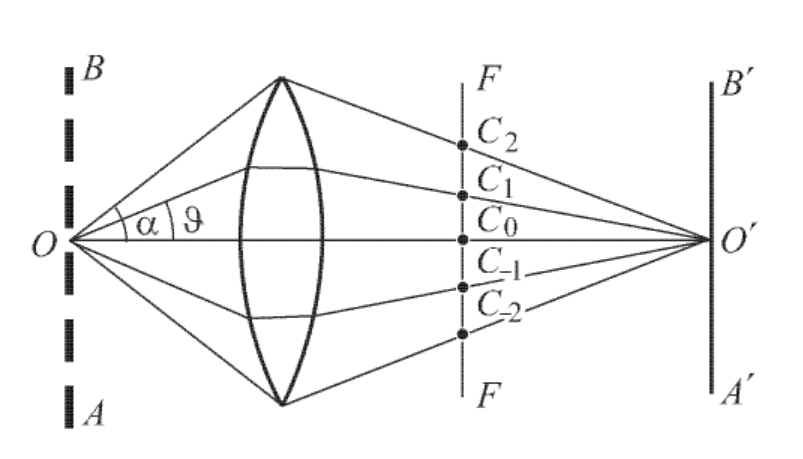
\includegraphics[width=0.5\textwidth]{figures/220.png}
    %\caption{}
    %\label{fig:}
\end{figure}
В фокусе мы получаем дифракционную картину из точек $C_k$, которую Аббе назвал первичным изображением объекта. Далее по Гюйгенсу-Френелю можно рассчитать световое поле далее за фокальной плоскостью, пусть они соберутся нашим объективом хоть где-то дальше, тогда получим \textit{вторичное изображение} или \textit{вторичную дифракцию}.


\Qsec{23}{Дифракция на периодических структурах с точки зрения фурье-оптики}


\begin{to_def}
    Объект называется \textit{абсорбционным}, если в различных местах обладает различной прозрачностью. Объект называется \textit{рефракционным}, если не поглощает света, но влиеяет на фазу. 
\end{to_def}


\Ssec{53}{Применение метода Рэлея}
\subsection{Применение метода Рэлея}


\textbf{Амплитудная решетка}. Есть решетка с щелями ширины $b$ и непрозрачных промежутков между ними ширины $a$. Начало координат в середине щели:
\begin{equation*}
    D_m = \frac{1}{d} \int_{-d/2}^{+d/2} D(x) e^{impx} \d x = 
    \frac{1}{d} \int_{-b/2}^{+b/2} e^{impx} \d x = \frac{b}{d} \frac{\sin \varkappa}{\varkappa},
    \hspace{5 mm}  
    \varkappa = \pi \frac{m b}{d}.
\end{equation*}
Что верно при малых углах дифракции, с $\cos \theta \approx 1$. Для спектра нулевого порядка $D_0 = b/d$, и $I_0 = (b/d)^2$, а полна $\sub{I}{прош} = b/d$, вообще верно, что
\begin{equation*}
    \frac{b}{d} = \frac{b^2}{d^2} + \frac{2}{\pi^2} \sum_{m=1}^{\infty} \frac{1}{m^2} \sin^2 \frac{\pi m b}{d}.
\end{equation*}
Относительная доля дифрагированного света
\begin{equation*}
    \frac{\sub{I}{прош} - I_0}{\sub{I}{прош}} = 1 - \frac{b}{d}.
\end{equation*}
Стоит помнить, что $d \sin \vartheta = m \lambda$. 





\textbf{Амплитудно-фазовая решётка.} Пусть есть участки длины $b$ с пропускаемостью $\beta$ и участки длины $a$ с пропускаемостью $\alpha$, где $\alpha$ и $\beta$ постоянны. 

Вычисение $D_m$ сводится к предыдущей задаче. Рассматриваемая решётка эквивалентна плоскопараллеьной решетке с пропусканием $\alpha$ и наложенной на неё дифракционной решетки пропускаемости $(\beta-\alpha)$. Так приходим к выражению
\begin{equation*}
    D_m = (\beta-\alpha) \frac{b}{d} \frac{\sin(\varkappa)}{\varkappa} + \alpha \delta_m, \hspace{5 mm} 
    \varkappa = \pi \frac{ m b}{d},
\end{equation*}
где $\delta_m = 1$ при $m=0$ и $\delta_m = 0$ при $m \neq 0$. В случае фазовой реешетки пропускаемости имеют вид $e^{i \rho}$, так как важна лишь разность фаз, то вполне можем положить $\alpha=1$ и $\beta=e^{i \rho}$. Тогда
\begin{align*}
    D_m &= (e^{i \rho}-1) \frac{b}{d} \frac{\sin\varkappa}{\varkappa}, \hspace{5 mm} m \neq 0, \\
    D_0 &= (e^{i \rho} -1) \frac{b}{d} + 1.
\end{align*}
Итого имеет дополнительный сдвиг фаз между спектром нулевого и спектрами всех прочих порядков. Можем его найти, посчитав
\begin{equation*}
    \arg \frac{D_m}{D_0} = \varphi, \hspace{5 mm} \tg \varphi = \frac{b+a}{b-a} \frac{\sin \rho}{1-\cos \rho}.
\end{equation*}
Введя на пути нулевого максимума пластину, меняющую фазу на $\varphi$ можем перейти к фазовым соотношениями, аналогичным амплитудной решетке, на основе этого и строится \textit{метод фазового контраста}. 

Стоит заметить, что при $a=b$ $\varphi =\pi/2$, а при $\rho \ll 1$  получим $\varphi \approx \pi/2$. 


\textbf{Эшелетт}. \red{Сивухин, страница 362.}






\Qsec{24}{Принципы пространственно фильтрации}

\Ssec{59}{Фазовый контраст}


% см. 53
% 400






\textbf{Идея фазового контраста}. Пусть два разных участка формируют векторы $\vc{A}$ и $\vc{B}$, при чём после фазовое решетки $|\vc{A}|$ близок к $|\vc{B}|$, но повернуты на некоторый угол (рис. \ref{fig:pfc59}, а).
\begin{figure}[ht]
    \centering
    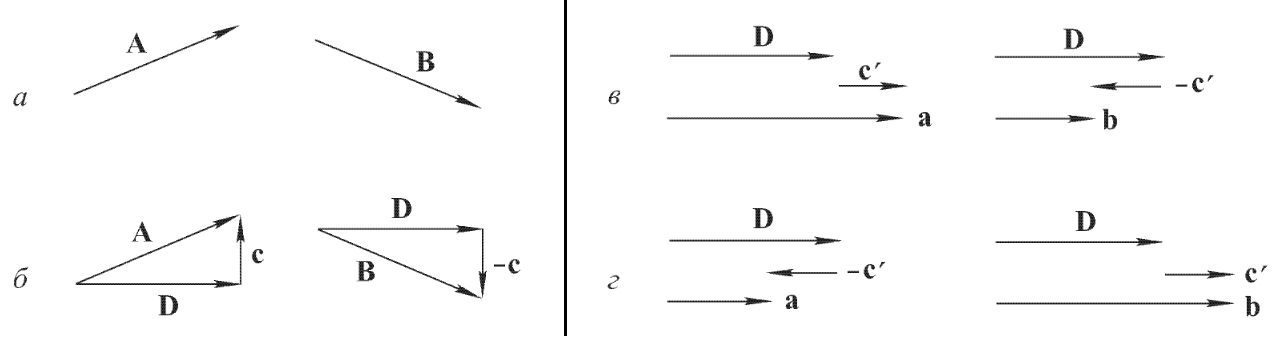
\includegraphics[width=0.65\textwidth]{figures/59_1.png}
    \caption{Метод фазового контраста}
    \label{fig:pfc59}
\end{figure}
Если повернуть $\vc{c}'$ и $\vc{c}$ на $\pi/2$, оставляя неизменным $\vc{D}$, то можем получить \textit{позитивный фазовый контраст} (в) и негативный фазовый контраст (г). 



\textbf{Реализация}. Прежде всего необходимо пространственно разделить волновые поля, представленные веткорами $\vc{c}$ и $\vc{D}$. Полное колебание имеет постоянную амплитуду на протяжении всей реешетки  и изображается вектором $\vc{D}$, оно даёт в фокальной плоскости центральный максимум, и только. 

Другое колебание представляется периодической функцией принимающую значения от $-\vc{c}$ до $\vc{c}$ на соседних участках, в среднем ноль, так что возбуждает только боковые максимумы, таким образом в фокальной плоскости объектива оба колебания окажутся пространственно разделенными. 

Поставив на пути либо центрального максимума, либо всех боковых максимумов прозрачную плоскопараллельную фазовую пластинке нужной тощины, можно ввести разность фаз в $\pi/2$ и так осуществить фазовый контраст. 


Стоит заметить, что раньше полная энергия на участках решётки была $2(D^2 + c^2)$, а после повтора $\vc{c}$ и $-\vc{c}$ энергия становится $(D+c)^2 + (D-c)^2$, то есть сохранятся, но перераспределяется. 







\Qsec{25}{Плоская голография}
\Ssec{54}{Про голографию из Сивухина}
\begin{wrapfigure}{r}{0.5\textwidth}
  \begin{center}
    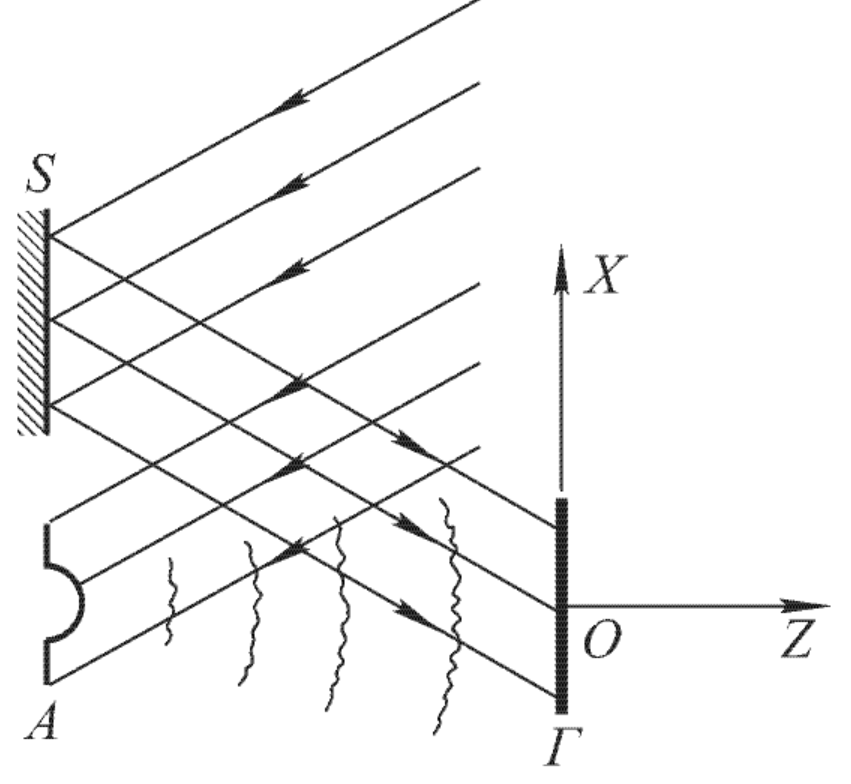
\includegraphics[width=0.28\textwidth]{figures/s54_1.png}
  \end{center}
\end{wrapfigure}
Идея голографии Габора заключается в том, что свет, попадая на объект рассеивается, и рассеянные лучи несут все информацию о форме и рельефе объекта. Однако для восстановления из таких лучей изображения нужна ещё информация о фазе изначально падавшего пучка, которую можно получить, если предварительно разделить этот пучок и часть его пустить на зеркало, чтобы переотразить в область, где мы хотим получать голограмму.
Пучок, рассеивающийся на предмете называется, называется \textit{предметным}, а несущий информацию о фазе -- \textit{опорным}.
Полученная картина на $\Gamma$ записывается, например на чувтсвительную пластину,  и называется голограммой, от греческого <<голог>> -- полный, <<графе>> -- пишу. Позже осветив её той же опорной волной можно получить восстановленное изображение объекта.

Запись голограммы -- очень тонкое дело. Необходимая степень монохроматичности света:
	$\boxed{\frac{\lambda}{\delta l} \gtrsim m}$,
	где $m$ -- максимальный порядок интерференции наблюдающийся при голографировнии.

Для хорошей установки и объекта с линейными размерами $L $ этот порядок можно оценить $\boxed{m \sim \frac{L}{\lambda}}$.
Таким образом должно быть: $\boxed{\delta\lambda < \frac{\lambda^2}{L}}$.

Требования к размеру источника тоже достаточно жестки: $\Delta x = \lambda/\alpha$, где $\alpha$ -- угол схождения крайних интерферирующих лучей. По порядку это что-то вроде $\alpha = h/l$, где $h$ -- ширина опорного пучка, а $l$ -- расстояния между предметом и голограммой. Таким образом $\boxed{\Delta x < \frac{\lambda l}{h}}$.

И так, о чем же сама голография. Представим поле рассеянной волны и отраженной:
\begin{equation*}
	u = a (\vc{r}) e^{i [\omega t - \Phi(\smallvc{r})]},
	\hspace{0.5 cm}
	v = b e^{i (\omega t - \smallvc{k} \smallvc{r})}.
\end{equation*}
Тут мы сделали упрощение, что поля не векторные, а скалярные, что для нас не сильно критично, и при таком упрощении $a(\vc{r})$, $\Phi(\vc{r})$ и $b$ будем считать вещественными. На пластинке $\Gamma$ интенсивность:
\begin{equation*}
	I  = v^* u + v u^* + v^* v + u^* u,
	\hspace{0.5 cm}
	I_0 = b a (x,y,0) e^{i[k_x x - \Phi(x,y,0)]} + b a (x,y,0) e^{-i[k_x x - \Phi(x,y,0)]} + b^2 + a^2(x,y,0).
\end{equation*}
где мы направили ось $Z$ перпендикулярно плоскости $\Gamma = XY$.

Допустим теперь, что нашу пластину, покрытую фотоэмульсией мы проявили и \href{https://youtu.be/y-MyaUcMkhs?t=252}{скопировали}, получив позитив голограммы. Пусть у позитива пропускаемость $D = I_0$, такую позитивную голограмму можно использовать для восстановления $u(\vc{r},t)$.
Для этого голограмму просвечивают таким же $v(\vc{r},t)$, он испытает дифракцию на голограмме типа как на диф-решетке. По методу Рэлея получим поле на выходе и будем искать решение волнового уравнения:
\begin{equation*}
	E_{\text{вых}} = D v (x,y,0) = I_{0} b e^{i (\omega t - k_x x)},
	\hspace{1 cm}
	\frac{\partial^2 E}{\partial x^2} + \frac{\partial^2 E}{\partial y^2} + \frac{\partial^2 E}{\partial z^2} + k^2 E = 0.
\end{equation*}
Будем искать решение для $E$ в виде $E = E_1 + E_2 + E_3 + E_4$, с граничными условиями:
\begin{equation*}
	\begin{aligned}
		&E_{1 \text{ вых}} = b^2 a(x,y,0) e^{i [\omega t - \Phi(x,y,0)]},\\
		&E_{2 \text{ вых}} = b^2 a(x,y,0) e^{i [\omega t + \Phi(x,y,0) - 2 k_x x]},	
	\end{aligned}
	\hspace{1 cm}
	\begin{aligned}
		&E_{3 \text{ вых}} = b^3 e^{i (\omega t - k_x x)},\\
		&E_{4 \text{ вых}} = b a^2(x,y,0) e^{i (\omega t - k_x x)}.
	\end{aligned}
\end{equation*}
Будем решать. Проще всего найти функцию $E_3 = b^3 e^{i (\omega t - \smallvc{k} \smallvc{r})} = b^2 v(\vc{r},t)$, это есть ни что иное, как опорная волна, распространяющаяся за голограмму.

Основной же интерес для голографии представляет собой поле $E_1$, $b$ -- постоянно, тогда:
\begin{equation*}
	E_1 = b^2 a (x,y,z) e^{i [\omega t - \Phi(x,y,z)]} = b^2 u (\vc{r},t).
\end{equation*}
Действительно, видим, что это волна, уходящая от голограммы. Она даст мнимое изображение объекта, в том же самом месте, в котором он находился до получения голограммы. 

Для нахождения $E_2$ сначала посмотрим на случай, когда опорный луч падает нормально плоскости голограммы, тогда $k_x = 0$, и немного другое граничное условие дадут решение
\begin{equation*}
	E_{2 \text{ вых}} = b^2 a(x,y,0) e^{i[\omega t + \Phi(x,y,0)]}
	\hspace{1 cm}
	\Rightarrow
	\hspace{1 cm}
	\tilde{E}_2 (x,y,z) = b^2 a (x,y,z) e^{i [\omega t + \Phi(x,y,z)]}.
\end{equation*}
Такая волна снова создаёт мнимое изображение, как и только что рассмотренная выше $E_1$, но она распространяется к голограмме, а не от нее, значит не может служить решением рассматриваемой нами задачи.
Чтобы починиться в уравнении Гельмгольца заменим $z \mapsto -z$
\begin{equation*}
	\frac{\partial^2 E}{\partial x^2} + \frac{\partial^2 E}{\partial y^2} + \frac{\partial^2 E}{\partial (-z)^2} + k^2 E = 0
	\hspace{1 cm}
	\Rightarrow
	\hspace{1 cm}
	E_2 = b^2 a(x,y,-z) e^{i[\omega t + \Phi(x,y,-z)]}.
\end{equation*}
Теперь волна идёт от голограммы, является решением нашей краевой задачи, и формирует таким образом действительное изображение.

\subsection{Голограмма Габора}
Рассмотрим простейшую голограмму -- голограмму точечного источника (рассеивателя), которая также называется \textit{голограммой Габора}. От него идут монохроматические сферические волны. А запись идёт тонкослойную пластину.
\begin{wrapfigure}{r}{0.6\textwidth}
     \centering
     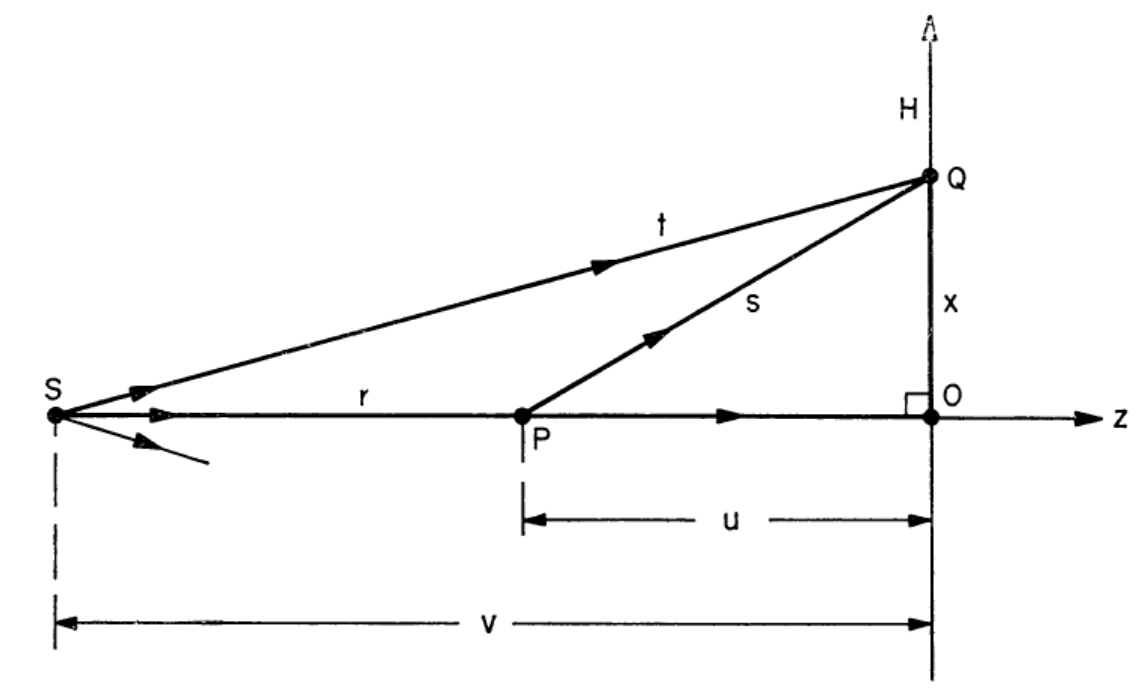
\includegraphics[width=0.5\textwidth]{figures/gabor_point.png}
     \caption{Голограмма Габора. Точечный источник $S$, находящийся на расстоянии $v$ от плоскости голограммы $H$, освещает рассеивающий центр $P$, находящийся на расстоянии $u$ от $H$. 
	}
     %\label{fig:}
 \end{wrapfigure}
Интерференция волн от $P$ и $S$ задается выражением: $I = I_1 + I_2 + 2 a_1 a_2 \cos (\varphi_2 - \varphi_1)$. Предполагая, что пропускание голограммы пропорционально $I$ получаем на голограмме интерференционную картину, зависящую от разности фаз $\Delta \varphi = \varphi_2 - \varphi_1$.

Пусть источник непрерывно излучает волну длинной $\lambda$ и чистотой $\nu$, фаза источника $\varphi = 2 \pi \nu t$.
Для скорости распространения света $c$ разность фаз в точке $Q$ в момент времени $t_Q$ на голограмме для лучей от источника и объекта будет:
\begin{equation*}
	\varphi_r - \varphi_s = \frac{2 \pi \nu}{c} (SPQ - SQ) = \Delta \varphi = \frac{2 \pi \Delta l}{\lambda}.
\end{equation*}
В тех случаях, когда $\Delta \varphi = 1$, то есть $\Delta l = n \lambda$ получаем максимумы по обозначениям рисунка и имея $x \ll u,v$ для опыта Габора:
\begin{equation*}
	\Delta l = (r+s) - t = (v - u + s) - t = v - u + \sqrt{u^2 + x^2} - \sqrt{v^2 + x^2} \approx v - u + u + \frac{x^2}{2 u} - v - \frac{x^2}{2 v} = \frac{x^2}{2}\left(\frac{1}{u} - \frac{1}{v}\right).
\end{equation*}
Вводя фокусное расстояние так называемой \textit{зонной пластинки} $f$ получаем:
\begin{equation*}
 	\frac{1}{f} = \frac{1}{u} - \frac{1}{v},
 	\hspace{1 cm}
 	\Rightarrow
 	\hspace{1 cm}
 	\Delta l = \frac{x_n^2}{2 f} = n \lambda.
 \end{equation*} 
 В силу осевой симметрии получаем таким образом радиусы колец $x_n$ максимальной яркости.

 Выражая $x_n$ получаем очень похожее на френелевские зоны выражение:
 \begin{equation*}
 	x_n = \sqrt{f \lambda} \cdot \sqrt{2 n}.
 \end{equation*}

 \begin{wrapfigure}{r}{0.5\textwidth}
     \centering
     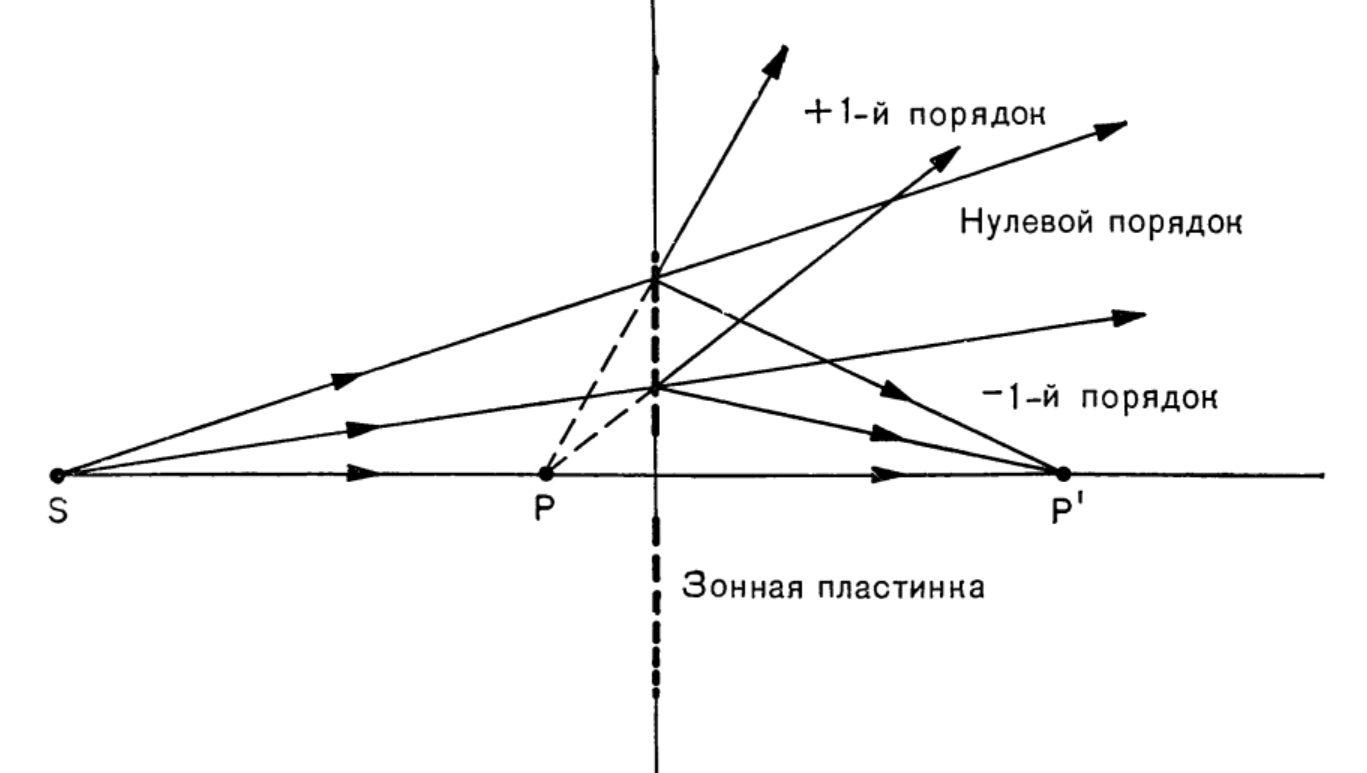
\includegraphics[width=0.5\textwidth]{figures/vosstan_gabor.png}
     \caption{Фокусирующие свойства зонной пластинки.}
     %\label{fig:}
 \end{wrapfigure}
 Изготовляя далее позитив голограммы получаем обнаруживаем, что он обладает соответственно теми же свойствами что и зонная пластинка Френеля, с той оговоркой, мы получили синусоидальную кривую пропускания, а не прямоугольную. При дифракции на нашей голограмме будут возникать только волны $\pm 1$ порядков, в то время как у Френеля и более высших порядков, но если последнего ограничить только по первым гармоникам, то картина получится идентичная.

 Мы говорили про $f$ -- фокус получившейся решетки. И для него получили выражение соответствующее формуле тонкой линзы.
 Таким образом имеем аналогию, что голограмма точечного объекта ведет себя подобно диф-решетке и подобно отрицательной линзе, создающей мнимое и действительное изображение. 

В более общем случае, как и в выводе из Сивухина, если представить протяженный объект как совокупность точек и пренебречь интерференцией волной от этах точек по сравнению с интерференцией с опорной волной, получим изображение объекта как суперпозицию зонных пластинок. И когда такая голограмма осветится опорной волной, каждая индивидуальная голограмма создаст мнимое изображения соответствующей точки объекта, а в процессе восстановления изображения точек создадут образ всего протяженного объекта.

И так, отвлекаясь от точки, все ещё можем записать разность хода между опорной и рассеянной волной:
\begin{equation*}
	\Delta l \frac{x^2 + y^2}{2} \left(\frac{1}{v} - \frac{1}{u}\right) = \frac{\rho^2}{2 f} = n \lambda.
\end{equation*}
Можно определить локальную пространственную частоту полос $\nu(\rho)$ следующим образом:
\begin{equation*}
	\nu(\rho) = \frac{\partial (\Delta \varphi)}{\partial\rho} \cdot \frac{1}{2 \pi} = \frac{\partial}{\partial \rho} \left(\frac{\Delta l}{\lambda_1}\right)
	\hspace{1 cm}
	\Rightarrow
	\hspace{1 cm}
	\nu(\rho) = \frac{\rho}{f \lambda}.
\end{equation*}
То есть по мере удаления от центра частота полос увеличивается. И при некотором $\rho$ частота $\nu$ может привысить разрешающую способность светочувствительной среды $\nu_m$.


\subsection{Голограмма с наклонным опорным пучком}
\begin{wrapfigure}{r}{0.5\textwidth}
     \centering
     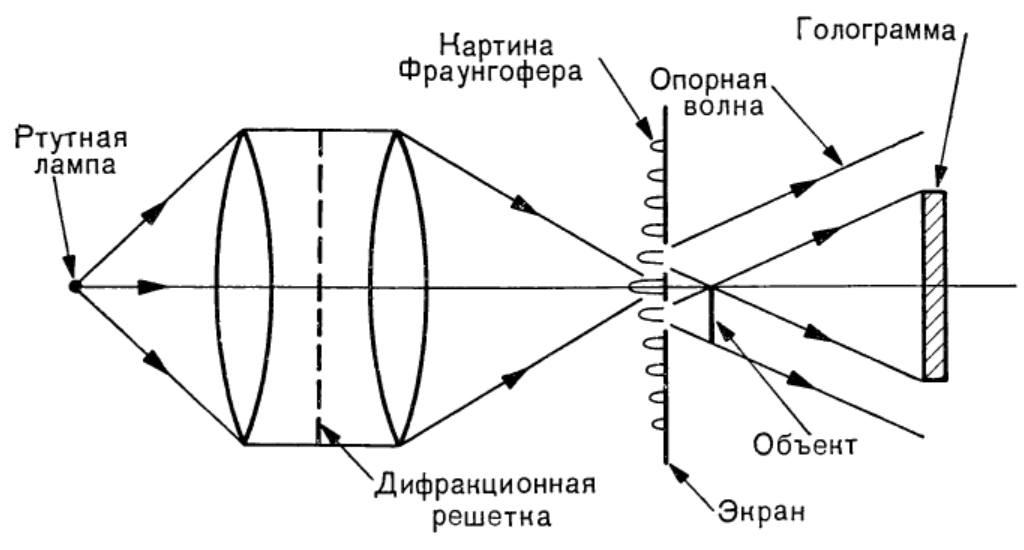
\includegraphics[width=0.5\textwidth]{figures/leyt_holo.png}
     \caption{Первоначальная схема получения внеосевых голограмм. (По Лейту и Упатниексу)}
     %\label{fig:}
 \end{wrapfigure}
Для получения осевых голограмм, как например, для точки из прошлого параграфа, требуется соблюдение ряда условий:
\begin{enumerate}
	\item объект должен состоять из малых непрозрачных участков на большом прозрачном фоне;
	\item с исходной голограммы приходится делать позитивный отпечаток;
	\item для устранения помех нужно в области действительного изображения голограммы загасить нежелательную дифракцию  от мнимого изображения объекта.
\end{enumerate}
Ученые, помучавшись с осевой геометрией системы с различными фильтрациями в итоге отказались от идеи осевой симметрии и перешли к наклонным опорным пучкам в голограммах, а именно это сделали \textit{Лейт и Упатниекс}. 

\begin{wrapfigure}{r}{0.5\textwidth}
     \centering
     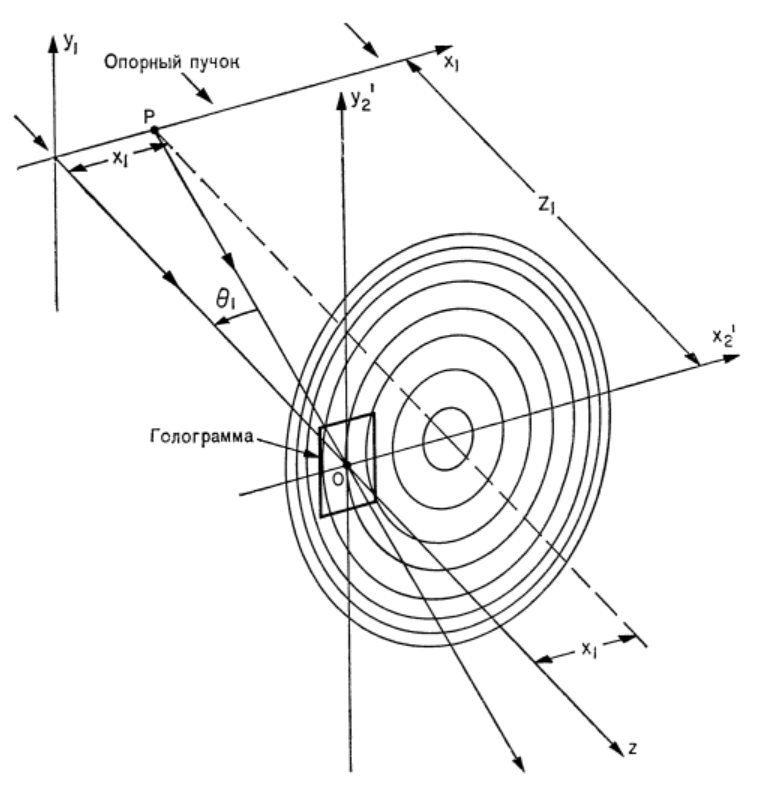
\includegraphics[width=0.5\textwidth]{figures/naclon_holo.png}
     \caption{Голограмма, образованная, точечным объектом $P$, расположенным не на оси, и аксиальной плоской опорной волной. }
     \label{fig:naclon}
 \end{wrapfigure}

Хочется сказать, что для внеосевой диаграмме, в соответствии с обозначениями на рисунке получаем разность хода, как и для осевого случая:
\begin{equation*}
	\Delta l = \frac{x_2^2 + y_2^2}{2} \left(\frac{1}{z_1} - \frac{1}{z_1}\right) - x_2 \left(\frac{x_r}{z_r} - \frac{x_1}{z_1}\right)
	 - y_2 \left(\frac{y_r}{z_r} - \frac{y_1}{z_1}\right) = n \lambda.
\end{equation*}
То есть уравнение окружности с координатами центра:
\begin{equation*}
	x_2 = \frac{z_1 x_r - z_r x_1}{z_1 - z_r}
	\hspace{0.5 cm}
	y_2 = \frac{z_1 y_r - z_r y_1}{z_1 - z_r}
	\hspace{1 cm}
	\Rightarrow
	\hspace{1 cm}
	\rho = x_2^2 + y_2^2 + \frac{2 n \lambda z_1 z_r}{z_1 - z_r}.
\end{equation*}
Частоту полос в направлении $x_2$ получим дифференцируя $\Delta l/\lambda$ по этому направлению при условии $x_r = y_r = y_1 = 0$ (см. рисунок \ref{fig:naclon}) и $z = \infty$. Получаем:
\begin{equation*}
	\frac{\partial}{\partial x_2} \frac{\Delta l}{\lambda} = \xi = \frac{x_2}{z_1 \lambda} + \frac{x_1}{z_1 \lambda}.
\end{equation*}
Сравнивая с частотой для осевой диаграммы наблюдаем такое же учащение полос при отхождении от $x_2 = x_\text{осевой} = 0$. А разность у них сохраняется равной $x_1/(z_1\lambda)$

Для того, чтобы на внеосевой голограмме была зарегистрирована интерференционная картина, нужно чтобы разрешающая способность светочувствительной среды была на $x_1/z_1 \lambda$ больше чем для осевой диаграммы. И для маленьких углов падения $x_r/z_r \approx \theta_r$ разность дастся как:
\begin{equation*}
	\left(\frac{x_1}{z_1} - \frac{x_r}{z_r}\right)\frac{1}{\lambda} \approx \frac{\theta_1 - \theta_r}{\lambda},
\end{equation*}
где $\theta_1$ -- средний угол между осью $z$и предметной волной.
\newpage

\Qsec{26}{Разноцветная голография}
\subsection{Условие Брегга-Вульфа}
\begin{figure}[ht]
    \centering
    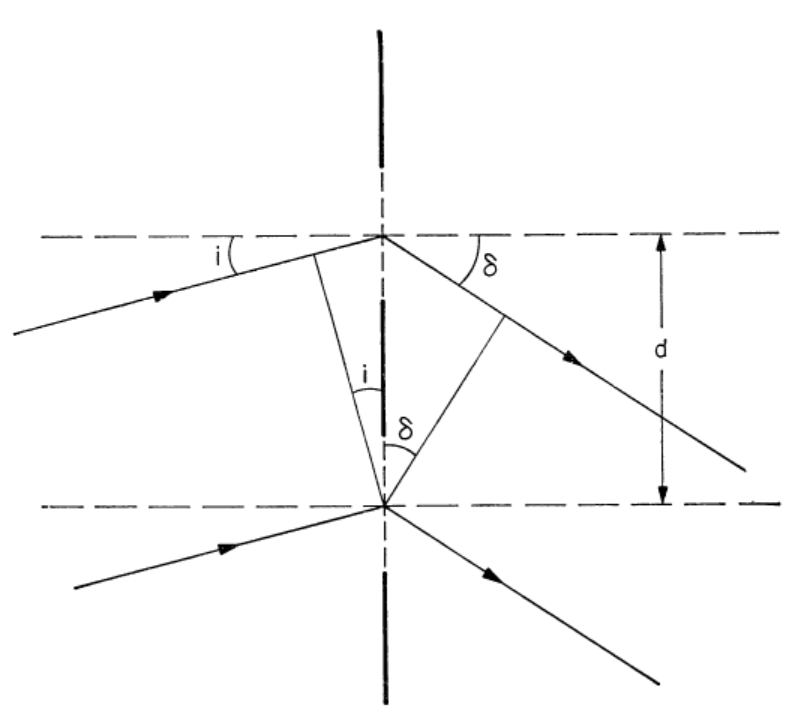
\includegraphics[width=0.4\textwidth]{figures/10_add_reshetka.png}
    \hspace{5 mm} 
    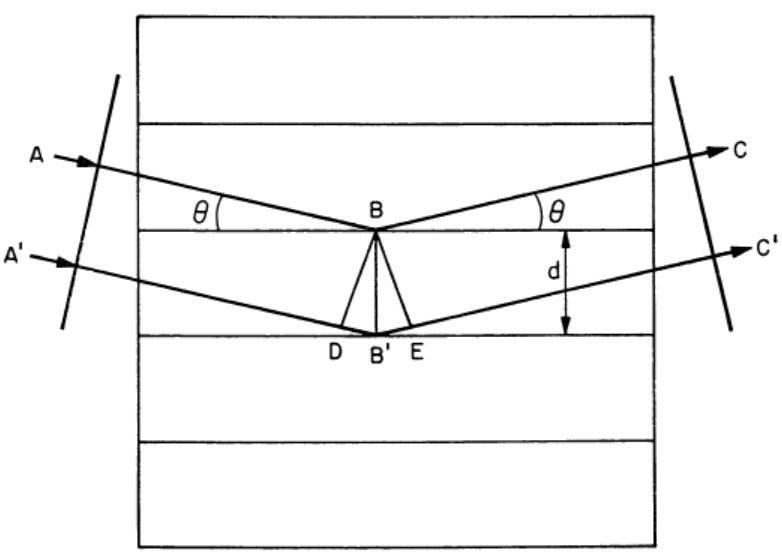
\includegraphics[width=0.4\textwidth]{figures/10_add_bregg.png}
    \caption{К формуле решетки плоской и объёмной}
    \label{fig:10_add}
\end{figure}

Помним формулу решетки, смотрим на левый рисунок(\ref{fig:10_add}), 
\begin{equation*}{}
	d (\sin i + \sin \delta) = \lambda,
\end{equation*}
 где ограничимся рассмотрением максимума первого порядка. 
Теперь рассмотрим правый рисунок(\ref{fig:10_add}) с объемной решеткой в разрезе.
Здесь аналогично интенсивность максимальна в том направлении, в котором волны складываются симфазно.

На рисунке $DB' + B'E = 2 d \sin \theta$, что с условием максимума даёт на закон Брегга-Вульфа:
\begin{equation*}
	2 d \sin \theta = m \lambda.
\end{equation*}
Таким образом получаем более жесткое условие на наблюдение $m$-го максимума дифракции.
Для объёмной решетки выбор угла падения определяет и длину волны и угол дифракции. 

Рассмотренная схема была впервые получена Бреггом и независимо от него Вульфом для ренгеновских лучей.
Напомним, что рентгеновский диапазон составляет от $10^{-3}$ нм до $100$ нм.
\textit{Жестким}  называют излучение с $\lambda < 0.2$ нм, оно обладает большой проникающей способностью в вещество.

Рассмотренная схема справа на рисунке(\ref{fig:10_add}) аналогична и по выводу для дифракции рентгеновских. Где уже нарисованные уровни, от которых происходит отражение -- \textit{атомные плоскости}, то есть плоскости в кристалле содержащее большое число атомов, до которых доходит рентгеновское излучение.
Отраженные же волны от кристалла рассматриваем так же, как отражение от разных атомных плоскостей.

Стоит заметит, что помимо максимумов, задаваемых условиям Брегга-Вульфа, есть ещё максимумы -- результаты отражения от разных слоев. Наиболее сильное отражение происходит от того слоя, где атомов больше.

Вдаваясь ещё в частности. Для монокристалла нужное найти положение в пространстве, при котором условие Брегга-Вульфа будет выполняться. В случае поликристалла и монохроматичного излучения найдется много кристаликов (плоскостей) для которых выполнится наше условие. На наборе таких плоскостей строится метод Дебая-Шеррера по изучению кристаллов в рентгеновском спектре.

\Qsec{27}{Поляризация света}

\Ssec{62}{Поляризованный и естественный свет}

\textbf{Общие слова}. 
Если взять немного йода с хинином, то получится герапатит, из которого часто делают \textit{поляроиды}. 
Рассмотрим систему из двух поляроидов: через оба поляроида пройдёт свет с электрическим вектором 
$\vc{E} \equiv \sub{\vc{E}}{$\parallel$}$, тогда интенсивность света после двух поляроидов:
\begin{equation*}
    I = I_0 \cos^2 \alpha,
\end{equation*}
что называют \textit{законом Малюса}. 

Рассмотрим два взаимноперпендикулярных колебания:
\begin{equation*}
    \left.\begin{aligned}
        x &= a \cos \omega t \\
        y &= b \cos (\omega t + \delta)
    \end{aligned}\right.    
    \hspace{0.5cm} \Rightarrow \hspace{0.5cm}
    \frac{x^2}{a^2} - 2 \frac{xy}{ab} \cos \delta + \frac{y^2}{b^2} = \sin^2 \delta.
\end{equation*}
Получили эллипс. Колебания с большей фазой -- \textit{опережающие},  с меньшей -- \textit{запаздывающие}. Соответсвенно, рассматривая скорости
\begin{equation*}
    \dot{x} = - \omega a \sin \omega t, \hspace{5 mm} 
    \dot{y} = - \omega b \sin(\omega t + \delta).
\end{equation*}
Тогда при $\delta < 0$ частица в $t=0$ движется вверх, а тогда описывает эллипс против часовой стрелки, а при $\delta > 0$ описывает эллипс по часовой стрелке. 

Для круговой поляризации можем заметить, что необходимо $\delta = \pm \pi/2$ и $a = b$, в частности можно различать правую и левую поляризацию. 

В частности, для монохроматического поля в векторной поле можем записать
\begin{align*}
    \vc{E} = \vc{A}_1(\vc{r}) \cos \omega t + \vc{A}_2 (\vc{r}) \sin \omega t,
\end{align*}
если $\vc{A}_1$ и $\vc{A}_2$ коллинеарны, то $\vc{E}$ поляризован линейной. Иначе же скажем, что $OX \parallel \vc{A}_1$ и $OY \parallel \vc{A}_2$, тогда получим
\begin{equation*}
     E_x = a_x (\vc{r}) \cos (\omega t + \delta_x), \hspace{5 mm} 
     E_y = a_y (\vc{r}) \cos (\omega t + \delta_y),
 \end{equation*} 
 что приводит как раз к сумме двух колебаний со сдвигом по фазе. 

\textit{Степень поляризации} света может быть определена, как
\begin{equation*}
    \Delta = \frac{I_{\bot}-I_{\parallel}}{I_\bot + I_\parallel}.
\end{equation*}
аналогично видности и не только. 


\textbf{Частично поляризованный свет}. Всякая монохроматическая волна по определению поляризована, обычно имеем дело с \textit{почти} монохроматическими, содержашимеся в некотором интервале $\Delta \omega$: рассмотрим такую волну с некоторой средней частотой $\omega$. Тогда поле в заданной точке пространства
\begin{equation*}
    \vc{E} = \vc{E}_0 (t) e^{-i \omega t},
\end{equation*}
где $\vc{E}_0 (t)$ -- медленно меняющаяся функция. Таким образом волна \textit{частично поляризована}. 

Наблюдаем почти всегда усредненное значение интенсивности, так что можем рассмотреть некоторый тензор
\begin{equation*}
    J_{\alpha \beta} = \overline{E_{0 \alpha} E_{0 \beta}^*},
\end{equation*}
имеющий всего четыре значения (здесь и далее считаем, что $\alpha,\, \beta = 1,\, 2$). Свёртка $J_{\alpha \beta}$  есть
\begin{equation*}
    J = J_{\alpha \alpha} = \overline{\vc{E}_0 \vc{E}_0^*},
    \hspace{5 mm} 
    \rho_{\alpha \beta} = \frac{J_{\alpha\beta}}{J},
\end{equation*}
таким образом приходим к \textit{поляризационному тензору}. Из определения понятно, что оба тензора эрмитовы, откду $\rho_{11}$ и $\rho_{22}$ вещественны, при чём $\rho_{11} + \rho_{22} = 1$, и $\rho_{21} = \rho_{12}^*$. Итого осталось три вещественных параметра. 

Пусть свет очень похож на поляризованный, тогда $J_{\alpha \beta} = J \rho_{\alpha \beta} E_{0 \alpha} E_{0 \beta}^*$, то есть компоненты некоторого постоянного вектора. Необходимо и достаточно $\det \rho_{\alpha \beta} = 0$. 

Аьтернатива: \textit{естественный} свет, тогда направления в плоскости $\bot$ распространению эквивалентны, тогда $\rho_{\alpha \beta} = \frac{1}{2} \delta_{\alpha \beta}$, тогда $\det \rho_{\alpha \beta} = 1/4$.

Итого возможны значения для $\det \rho_{\alpha \beta} \in [0, 1/4]$, соответсвенно \textit{степенью поляризации} назовём величину $P$ равную
\begin{equation*}
    P \overset{\mathrm{def}}{\colon} \ \ \det \rho_{\alpha \beta} = \frac{1}{4} \left(1-P^2\right), \hspace{5 mm} 
    P \in [0, 1]. 
\end{equation*}
Да, можно и так. 


Произвольный тензор $\rho_{\alpha \beta}$ может быть разложен на две части: симметричную и антисимметричную, из них первая $S_{\alpha \beta} = \frac{1}{2} \left(\rho_{\alpha \beta} + \rho_{\beta \alpha}\right)$ -- вещественная в силу эрмитовости $\rho_{\alpha \beta}$, антисимметричная же части чисто мнима, которая сводится к псевдоскаляру
\begin{equation*}
    \frac{1}{2}\left(\rho_{\alpha\beta} - \rho_{\beta \alpha}\right) = - \frac{i}{2} e_{\alpha \beta} A,
\end{equation*}
где $A$ -- вещественный псевдоскаляр. Итого, поляризационный тензор представим в виде
\begin{equation*}
    \rho_{\alpha \beta} = S_{\alpha \beta} - \frac{i}{2} e_{\alpha \beta} A.
\end{equation*}
Для поляризованной по кругу волны $\vc{E}_0 = \const $, тогда $A = \pm 1$, а $S_{\alpha \beta} = \frac{1}{2} \delta_{\alpha \beta}$, а вот для линейно поляризованной волны $A = 0$. Вообще $A$ -- степень круговой поляризации, $A \in [-1, + 1]$, где предельные значения -- правая и левая поляризации. 

Вектор $S_{\alpha \beta}$ может быть сведен к гланым осяи с главными значениями $\lambda_1$ и $\lambda_2$, направления которых нормальны, при чём $\lambda_1 + \lambda_2 = 1$. Тогда
\begin{equation*}
    S_{\alpha \beta} = \lambda_1 n_\alpha^{(1)} n_{\beta}^{(1)} + \lambda_2 n_\alpha^{(2)} n_\beta^{(2)}.
\end{equation*}
При $A = 0$ каждое из слагаемы -- произведения постоянного вещественного веткора $\sqrt{ \lambda_1} \vc{n}^{(1)}$ и $\sqrt{ \lambda_2} \vc{n}^{(2)}$, получается соответсвет линейно поляризованному свету, независимых \textit{некогерентных} волн. В общем же случае свет может быть представлен как наложение двух некогернтных эллиптически поляризованных волн, эллипсы которых нормальны. 


Пусть $\varphi$ -- угол между $Oy$ и $\vc{n}^{(1)}$, тогда
\begin{equation*}
    \vc{n}^{(1)} = (\cos \varphi,\, \sin \varphi)\T, \hspace{5 mm} 
    \vc{n}^{(2)} = (-\sin \varphi,\,  \cos \varphi).
\end{equation*}
Вводя величину $l = \lambda_1 - \lambda_2$ можем представить компаненты тензора в виде
\begin{equation*}
    S_{\alpha \beta} = \frac{1}{2} \begin{pmatrix}
        1 + l \cos 2 \varphi & l \sin 2 \varphi  \\
        l \sin 2 \varphi & 1 - l \cos 2 \varphi  \\
    \end{pmatrix}.
\end{equation*}
Итого можем в качетсве параметров выбрать $A$ -- степень круговой поляризации, $l$ -- степень максимальной линейной поляризации, $\varphi$ -- угол межу $\vc{n}^{(1)}$ и осью $Oy$. 

Но можно выбрать параметры удобнее:
\begin{equation*}
    \xi_1 = l \sin 2 \varphi,
    \hspace{5 mm} 
    \xi_2 = A,
    \hspace{5 mm} 
    \xi_3 = l \cos 2 \varphi,
    \hspace{5 mm} 
    \text{---\  \textit{параметры Стокса}}.
\end{equation*}
Тогда поляризационный тензор примет вид
\begin{equation*}
    \rho_{\alpha \beta} = \frac{1}{2} \begin{pmatrix}
        1+\xi_3 & \xi_1 - i \xi_2  \\
        \xi_1 + i \xi_2 & 1-\xi_3  \\
    \end{pmatrix},
    \hspace{5 mm} 
    \xi_1, \xi_2, \xi_3 \in [-1, +1].
\end{equation*}
где $\xi_3$ -- линейная поляризации вдоль $y$ и $z$, $\xi_1$ -- поляризации вдоль направлений под углом $\pi/4$, $\xi_2 = A$. Определитель 
\begin{equation*}
    \det \rho_{\alpha \beta} = \frac{1}{4}\left(1 - \xi_1^2 - \xi_2^2 - \xi_3^2\right),
    \hspace{5 mm} 
    P = \sqrt{\xi_1^2 + \xi_2^2 + \xi_3^2},
\end{equation*}
что очень удобно. Кстати, $\xi_2 = A$ и $\sqrt{\xi_1^2 + \xi_3^2} = l= \lambda_1 - \lambda_2$ -- инваринантны относительно преобразований Лоренца, что также очень логично. 




\Qsec{28}{Кристаллооптика I}


\Ssec{75}{Плоские волны в кристаллах}
Поведение света всё также описывается уравнениями Максвелла
\begin{equation*}
    \rot \vc{H} = \frac{1}{c} \dot{\vc{D}},
    \hspace{5 mm} 
    \rot E = - \frac{1}{c} \dot{\vc{H}},
\end{equation*}
однако усложняются материальные уравнения:
\begin{equation*}
    D^j = \varepsilon_i^j E^i,
\end{equation*}
где $\varepsilon_{ij}$ -- \textit{тензор диэлектрической проницаемости}, или \textit{диэлектрический тензор}.
% Такая анизотропия приводит к неколлинеарности $\vc{D}$ и $\vc{E}$.

Рассмотрим плоские монохроматические волны вида
\begin{equation*}
    \vc{A} = \vc{A}_0 e^{i(\omega t - \smallvc{k} \cdot \smallvc{r})}, 
\end{equation*}
где $\vc{A} \in \{\vc{E},\, \vc{H},\, \vc{D}\}$. Понятно, что
\begin{equation*}
    \rot \vc{H} = -i \left[\vc{k} \times  \vc{H}\right],
    \hspace{5 mm} 
    \partial_t \vc{D} = - i \omega \vc{D}, \hspace{5 mm} \ldots
\end{equation*}
Подставив это в уравнения Максвелла, вводя верно волновой нормали $\vc{N} = \frac{v}{\omega} \vc{k}$, получаем
\begin{equation*}
    \vc{D} = - \frac{c}{v} \left[\vc{N} \times \vc{H}\right],
    \hspace{5 mm} 
    \vc{H} = \frac{c}{v} \left[\vc{N} \times \vc{E}\right],
\end{equation*}
где $v$ -- нормальная скорость волны. 

Актуально, как никогда, значение вектора Пойтинга
\begin{equation*}
    \vc{S} = \frac{c}{4\pi}\left[\vc{E} \times \vc{H}\right].
\end{equation*}

\begin{to_lem}
    Вектор пойтинга $\vc{S}$ определяет направление световых лучей, то есть $S \parallel \vc{u} = d_{\smallvc{k}} \omega$.
\end{to_lem}

Стоит заметит, что в кристаллая $\vc{S}$ и $\vc{N}$ не совпадают по направлению. 
Однако, как видно из формул, плоские волны в кристалле поперечн в отношении векторов $\vc{D}$ и $\vc{H}$. Вектора $\vc{E},\, \vc{D},\, \vc{N},\,  \vc{S}$ лежат в плоскости, перпендикулярной к вектору $\vc{H}$. 

Получается, что если $\vc{E}$ и $\vc{D}$ не сонаправлены, то зная направление $\vc{E}$ мы знаем направление и $\vc{D}$, а тогда и $\vc{H}$, и $\vc{N}$, $\vc{S}$ соответственно тоже. 
При $\vc{E} \parallel \vc{D}$ любая прямая $\bot \vc{E}$ может служить направлением магнитного поля. 
Подставляя $\vc{H}$ в $\vc{D}$ можем найти
\begin{equation*}
    \vc{D} = \frac{c^2}{v^2} \vc{E} - \frac{c^2}{v^2} \left(\vc{N} \cdot \vc{e} \right) \vc{N},
\end{equation*}
и, т.к. $(\vc{D} \cdot \vc{N})=0$, то скалярно умножая на $\vc{D}$ находим
\begin{equation*}
    v^2 = c^2 \frac{(\vc{D} \cdot \vc{E})}{D^2}.
\end{equation*}
Таким образом вектор $\vc{E}$ в кристале является \textit{главным}.


\Ssec{76}{Оптически одноосные кристаллы}
\subsection{Оптически одноосные кристаллы}

\begin{to_def}
    \textit{Оптически одноосными} называют кристаллы, свойства которых обладают симметрей вращения относительно некоторого направления, называемого \textit{оптической осью кристалла}.
\end{to_def}

Разложим $\vc{E}$ и $\vc{D}$ на составляющие параллельные оптической оси, и нормальный к ней, тогда
\begin{equation*}
    \vc{D}_\parallel = \varepsilon_\parallel \vc{E}_\parallel,
    \hspace{5 mm} 
    \vc{D}_\bot = \varepsilon_\bot \vc{E}_\bot,
\end{equation*}
где $\varepsilon_\parallel$ и $\varepsilon_\bot$ -- продольная и поперечные диэлектрические проницаемости кристалла. Плоскости, в которой лежат оптическая ось кристалла и нормаль $\vc{N}$, называется \textit{главным сечением кристалла}. 


\begin{to_def}
    Если электрический вектор $\vc{D}$ перпендикулярен к главному сечению, то скорость волны не зависит от направдения её распространения, такая волна называется \textit{обыкновенной}.
\end{to_def}

Тогда $\vc{D} \equiv \vc{D}_\bot$, тогда и $\vc{D} = \varepsilon_\bot \bar{E}$, соответственно 
\begin{equation*}
    \vc{D} = \varepsilon_\bot \vc{E},
    \hspace{0.5cm} \Rightarrow \hspace{0.5cm}
    \left.\begin{aligned}
        D &= H \textstyle \frac{c}{v} \\
        H &= E \textstyle \frac{c}{v}
    \end{aligned}\right.
    \hspace{5 mm} \Rightarrow \hspace{5 mm} 
    v = v_\bot \equiv \sub{v}{o} = \frac{c}{\sqrt{\varepsilon_\bot}}.
\end{equation*}

\begin{to_def}
    Если электрический вектор $\vc{D}$ лежит в главном сечении, то скорость волны зависит от направления распространенияЮ и такую волну называют \textit{необыкновенной}.
\end{to_def}

Вектор $\vc{E}$ в таком случае также лежит в главном сечении, и $\vc{E} = \vc{e}_N + \vc{E}_D$. В таком случае, верно
\begin{equation*}
    \vc{H} = \frac{c}{v} \left[\vc{N} \times \vc{E}_D\right],
    \hspace{5 mm} 
    E_D = \frac{\vc{E} \cdot \vc{D}}{D} = \frac{E_\parallel D_\parallel + E_\bot D_\bot}{D} = \frac{1}{D} \left(
        \frac{D_\parallel^2}{\varepsilon_\parallel} + \frac{D_\bot^2}{\varepsilon_\bot}.
    \right)
\end{equation*}
Соответсвующие проекции можно заменить на $D \sin \alpha$, где $\alpha$ -- угол между оптической осью и волновой нормалью. Вводя $\frac{1}{\varepsilon} = \frac{N^2_\bot}{\varepsilon_\parallel}+\frac{N^2_\parallel}{\varepsilon_\bot}$ можем перейти к
\begin{equation*}
    E_D = D\left(
        \frac{\sin^2 \alpha}{\varepsilon_\parallel} + \frac{\cos^2 \alpha}{\varepsilon_\bot}
    \right) = \frac{D}{\varepsilon},
    \hspace{5 mm} 
    H = \frac{c}{v} E_D,
    \hspace{0.5cm} \Rightarrow \hspace{0.5cm}
     v = \frac{c}{\sqrt{\varepsilon}} = c \sqrt{\frac{N^2_\bot}{\varepsilon_\parallel}+\frac{N_\parallel^2}{\varepsilon_\bot}}\equiv v_\parallel.
\end{equation*}


Когда $N_\bot =0$, то понятно, что $v = c/\sqrt{\varepsilon_\bot} = v_\bot = \sub{v}{o}$, -- нет разницы между обыкновенной и необыкновенной. В случае $N_\parallel = 0$  верно, что $v = \sub{v}{e} \overset{\mathrm{def}}{=} c/\sqrt{\varepsilon_\parallel}$. 

Термин оптическая ось введен для обозначения прямой, вдоль которой обе волны распростаняются с одинаковыми скоростями, и таким прямых в общем случае, поэтому кристалл называется \textit{оптически двуосным}. В рассмотренном частном случае оси совпали, и получился \textit{оптически одноосный} кристалл.


\begin{to_lem}
    В общем случае волна, вступающая в кристалл изотропной среды, разделяется внутри кристалла на две линейно поляризованные волны: обыкновенную, вектор электрической индукции которой перпендикулярен к главному сечению,
    и необыкновенную с вектором электрической индукции, лежащим в главном сечении.
\end{to_lem}

\textbf{Про показатели преломления}. В кристаллая верны законы преломления для \textit{волновых нормалей}: их направления подчиняются закону Снеллиуса
\begin{equation*}
    \frac{\sin \varphi}{\sin \psi_\bot} = n_\bot,
    \hspace{5 mm} 
    \frac{\sin \varphi}{\sin \psi_{\parallel}} = n_{\parallel},
\end{equation*}
где $n_\bot$ и $n_\parallel$ -- показатели прелоления обыкновенной и необыкноуенной волн, т.е.
\begin{equation*}
    n_\bot = \frac{c}{v_\bot} = \sub{n}{o},
    \hspace{5 mm} 
    n_\parallel = \frac{c}{v_\parallel} = \left(\frac{N^2_\bot}{\varepsilon_\parallel}+\frac{N^2_\parallel}{\varepsilon_\bot}\right)^{-1/2}.
\end{equation*}
Постоянная $\sub{n}{o}$ называется \textit{обыкновенным показателем преломления}. Когда необыкновенная волна распространяется перпендикулярно к оптической оси $(N_\bot=1)$, 
\begin{equation*}
    n_\parallel = \sqrt{\varepsilon_\parallel} \overset{\mathrm{def}}{=} \sub{n}{e}.
\end{equation*}
Величина $\sub{n}{e}$ -- \textit{необыкновенный показатель преломления кристалла}. 


\textbf{Двойное лучепреломление}. При преломлении на первой поверхности пластинки волна внутри кристалла разделяется на обыкноыенную, и необыкновенную. Эти волны поляризованы во взаимно перпендикулярных плоскостях и распространяются внутри пластинки в разных направлниях и с разными скоростями. Таким образом можно добиться пространственного разделения двух лучей. 
% рис 1


\Qsec{29}{Кристаллооптика II}


\Ssec{78}{Анализ поляризованного света}



\textbf{Анализ поляризованного света}. \textit{Пластинка в четверть волны} ($\lambda/4$), вносит дополнительную разность фаз в $\pi/2$ между проходящими через неё лучами, поляризованными во взаимно перпедикулярных плоскостях. 

 

% 
\textbf{Лучи и волновые нормали.}

 %- лучи и волновые нормали


\Ssec{90}{Эффект Керра: двойное преломление в электрическом и магнитном полях}


\subsection{Двойное преломление в электрическом и магнитном полях (эффект Керра)}

\textit{Электрический эффект Керра состоит в том}, \textit{что многие изотропные тела при введении в постоянное электрическое поле становится оптически анизотропным}. В частности, ведут себч как одноосные двупреломляющие кристаллы, оптическая ось которых параллельна приложенному электрическому полю. 


Пусть внешнее поле $\vc{E}_0$ \textit{однородно}. Понятно, что $\sub{n}{e}-\sub{n}{o}$ зависит от $\vc{E}_0$ в виде
\begin{equation*}
    \sub{n}{e} - \sub{n}{o} = q E_0^2,
\end{equation*}
для малых полей, где $q$ зависит только от вещества и от $\lambda$. В таком случае разность фаз между обыкновенной и необыкновенными лучами будет
\begin{equation*}
    \varphi = \frac{2\pi}{\lambda}(\sub{n}{e} - \sub{n}{o}) l = 2 \pi B l E^2,
\end{equation*}
где $l$ -- толщина образца, а $B \equiv q/\lambda$ -- \textit{постоянная Керра}. \textbf{Явление Керра объясняется анизотропией самих молекул.} 

Для эффекта Керра в газах, в случае полностью анизотропных молекул, можно показать, что при $\vc{E} \parallel \vc{E}_0$ показатель преломления будет \textit{необыкновенным}, тогда
\begin{equation*}
    n = 1 + \frac{2\pi}{3} N \beta,
\end{equation*}
где $\beta$ -- поляризуемость молекулы вдоль оси молекулы. Если же $\vc{E} \bot \vc{E}_0$, то  показатель преломления будет обыкновенным, и
\begin{equation*}
    \sub{n}{o} = 1 + 2 \pi N \beta \langle \sin^ \vartheta \rangle,
\end{equation*}
где $\vartheta$ -- угол\footnote{
    \red{Дописать}.
}  между $\vc{E}$ и $\vc{s}$.

Забавный факт: из полученных соотноешний можем получить
\begin{equation*}
    \frac{\sub{n}{e}-n}{\sub{n}{o}-n} = -2,
\end{equation*}
что выполняется для большинства веществ. 


Проводя некоторый аккуратны расчёт можем получить выражение для постоянной Керра:
\begin{equation*}
    \sub{n}{e} - \sub{n}{o} = \frac{n-1}{5} \frac{\beta}{kT} E_0^2.
\end{equation*}


\Ssec{91}{Эффект Поккельса (линейный электрооптический)}



Рассмотрим \textit{ангармонический осциллятор}  при наличии внешнего постоянного электрического поля $E_0$ 
\begin{equation*}
    \ddot{r} + 2 \gamma \dot{r} + \omega_0^2 r + \beta r^2 = -\frac{e}{m}E_0,
\end{equation*}
где $\beta$ -- постоянная. Считая $r = r_0 + q$ можем перейти к уравнению с новой частотой
\begin{equation*}
    \ddot{q} + 2 \gamma \dot{q} + (\omega_0^2+ 2\beta r_0) q =0,
\end{equation*}
откужа видно изменение частоты колебания на 
\begin{equation*}
    \Delta \omega_0^2 = -\frac{2 e \beta}{m \omega_0^2} E_0^2.
\end{equation*}
Смещение собственных частот меняет кривую дисперсии, т.е. показатель преломления $n$ среды. В простейшем случае, когда $\omega_0$ одна (см. \S 84), изменение $n$ определяется выражением
\begin{equation*}
    \Delta n = \frac{\partial n}{\partial \omega_0^2} \Delta \omega_0^2 = - \frac{\partial n}{\partial \omega_0^2} 
    - \frac{\partial n}{\partial \omega_0^2} \frac{2e\beta}{m \omega_0^2} E_0 = 
    \frac{\partial n}{\partial \omega} \frac{e\beta}{m \omega \omega_0^2} E_0.
\end{equation*}
При фиксированном внешнем $\vc{E}_0$ величина $\Delta n$ зависит от направления распространения света.
Это сказывается на двойном преломлении среды. \textit{Изменеие двойного преломления вещества из-за смещения собственной частоты во внешнем электрическом поле называется электрооптическим эффектом Поккельса}.

В этом эффекте изменения пропорциональны первой степени $E_0$. \textit{Эффект Поккельса может наблюдаться только в 
кристаллах, не обладающих центром симметрии.} Устройство, основанное на эффекте Поккельса, называют \textit{ячейкой Поккельса}. 

Она представляет собой кристалл, помещаемый между двумя скрещенными николями. 
Такое устройство действует так же, как и ячейка Керра. Николи
не пропускают свет, когда нет внешнего электрического поля,
но при наложении такого поля пропускание появляется. 
Необходимо, чтобы кристалл до наложения внешнего электрического
поля не давал двойного преломления. Этого можно достигнуть,
если взять оптически одноосный кристалл, вырезанный 
перпендикулярно к оптической оси, а свет направить вдоль этой оси.
Внешнее поле Eq может быть направлено либо перпендикулярно
(поперечный модулятор света), либо параллельно 
распространению света (продольный модулятор).





\Ssec{94}{Вращение плоскости поляризации}
\subsection{Вращение плоскости поляризации}


Если линейно поляризованный свет проходит через плоскопараллельный слой вещества, то в некоторых случаях плоскость поляризации света оказывается повернутой относительно своего исходного положения. Это явление называется \textit{вращением плоскости поляризации} или оптической активностью. Если вещество не находится во внешнем магнитном поле, то оптическая активность и вращение плоскости поляризации называются \textit{естестыенными}. В противоположнос случае говорят о \textit{магнитном вращении плоскости поляризации}, или \textit{эффекте Фарадея}. 


Вращение против часовов -- \textit{положительное}, по часовой -- \textit{отрицательное}. Это свойство, как и в случе с шурупом, не зависит от того, в каком из двух прямо противоположных напралний распространяетя свет\footnote{
    Если свет заставить пройти туда и обратно через естественно-активное вещество, отразив его от
    зеркала, то плоскость поляризации возвратится к своему исходисходному направлению.
} . 


В области прозрачности и малого поглощения эта история хорошо согласуется с опытом формула Друде
\begin{equation*}
    \xi = \alpha L,
    \hspace{5 mm} 
    \alpha = \sum_i \frac{B_i}{\lambda^2-\lambda_i^2},
\end{equation*}
где $B_i$ -- постоянные, $\lambda_i$ -- длины волн, соответсвующие собтсвенным чатсота рассматриваемого вещества. 



По Френелю вращение плоскости поляризации -- проявление \textit{кругового двойного лучепрпеломления}. Две волны, которые могут распространятся в оптически активной среде с разными скоростями, поляризованы \textit{по кругу}: по левому и по правому.

Покажем достаточность такого предположения:
\begin{equation*}
    \left.\begin{aligned}
        E_x &= A \cos \xi \cos (\omega t - k z), \\
        E_y &= A \sin \xi \cos (\omega y - k z),
    \end{aligned}\right.
    \hspace{5 mm} 
    \xi = - \alpha z,
    \hspace{0.5cm} \Rightarrow \hspace{0.5cm}
    \left.\begin{aligned}
        E_x &= \textstyle \frac{A}{2} \cos(\omega t - k z + \alpha z) + \textstyle \frac{A}{2} \cos(\omega t - k z - \alpha z), \\
        E_y &= \textstyle \frac{A}{2} \cos(\omega t - k z + \alpha z + \pi/2) + \textstyle \frac{A}{2} \cos(\omega t - kz - \alpha z - \pi/2).
    \end{aligned}\right.
\end{equation*}
Разложим полученную волну на две: $\vc{E} = \sub{\vc{E}}{п} + \sub{\vc{E}}{л}$, где для  $ \sub{\vc{E}}{п}$ и $\sub{\vc{E}}{л}$ имеет смысл ввеси $\sub{k}{п} = k-\alpha$  и $\sub{k}{л} = k + \alpha$. Полученные волны соответствуют правой и левой круговой поляризации. Скорости этих волн определяются выражениями
\begin{equation*}
    \sub{v}{п} = \frac{\omega}{k-\alpha}, \hspace{5 mm} \sub{v}{л} = \frac{\omega}{k+\alpha},
\end{equation*}
и соответсвующие покзатели преломления $n = c/v$. Подробнее,
\begin{equation*}
    \sub{n}{r} = \frac{c}{\sub{v}{r}} = \frac{c}{\omega}(k-\alpha),
    \hspace{5 mm} 
    \sub{n}{l} = \frac{c}{\sub{v}{l}} = \frac{c}{\omega}(k+\alpha),
    \hspace{0.5cm} \Rightarrow \hspace{0.5cm}
    \alpha = \frac{\omega}{2c}(\sub{n}{l}-\sub{n}{r}).
\end{equation*}




Френель выдвинул гипотезу, что возможно независимое распространения поляризованных по кругу волн, с сохранением поляризации, которую подтвердил эксперементально. Тем самым задача объяснения вращения плоскости поляризации была сведена к задаче объяснения кругового двойного лучепреломления.

Поляризованные по кругу в противоположных направлениях
волны в окрестности полос или линий поглощения могут 
отличаться не только скоростями распространения, но и 
коэффициентами поглощения. Тогда они выйдут с различными 
амплитудами. Если падающий свет был поляризован линейно, то 
выходящий будет поляризован эллиптически. Это явление 
называется круговым дихроизмом. 

\Ssec{95}{Эффект Фарадея: магнитное вращение плоскости поляризации }
Опыты Фарадея показали, что при наличии внешнего магнитного поля вдоль оптической оси системы, угол поворота зависит от длины пути $l$ и напряженноести внешнего поля $B$, как
\begin{equation*}
    \xi = R\, l B,
\end{equation*}
де $R$ -- \textit{постоянная Верде}, или \textit{магнитная вращательная способность}. 

При внесении в магнитное поле $\vc{B}$ у осцилляторов вещества появляются две новые резонансные частоты $\omega_0 + \Omega$ и $\omega_0 - \Omega$, где $\Omega$ -- ларморовская частота. Эти собственны частоты проявляеются не только в испускании (\textit{прямой эффект Зеемана}), но и в поглощении света (\textit{обратный эффект Зеемана}). 

Нормальные волны, которые могут распространятся вдоль магнитного поля, поляризованы по кругу. Когда направления распространения света и магнитного поля совпадают, большей частоте $\omega_+ = \omega_0 + \Omega$ соответсвует вращение по, а меньшей $\omega_-$ -- против часовой стрелки, если смотреть в направлении магнитного поля. Так как $\omega_+$ и $\omega_-$ различны, то происходит сдвиг фаз волн, а соответсвенно, и повород плоскости поляризации на гол
\begin{equation*}
    \xi = \frac{\omega l}{2c} (n_- - n_+) = \frac{\pi l}{\lambda} (n_- - n_+).
\end{equation*}

Если построить $n_- - n_+$, то можно увидеть, что, как и в случае ларморовского вращения $\Omega$, вращение плоскости поляризации определяется только направлением магнитного поля $\vc{B}$ и не зависят от направления распространения света.  При изменение на противоположное направления распространеняи света не изменятся, в противоположность естественного вращения. 

Вообще, в эффекте Фарадея, воспользовавшись формулой Зеемана можно получить \textit{формулу Беккереля} для постоянной Верде:
\begin{equation*}
    R = - \frac{e}{2 mc^2} \lambda \frac{d n}{d \lambda},
\end{equation*}
где $m$ -- масса электрона, $e > 0$ -- его абсолютный заряд.  


Ещё можно было бы поговорить про \textit{эффект Макалюзо и Корбино}, объясненный Фохтом, но оставим это на светлое будущее. 




\Qsec{30}{Нелинейная оптика I}


\Ssec{123}{Нелинейная поляризацим среды}
\subsection{Нелинейная поляризацим среды}

% § 91, 99, 100).

При распространении света в среде нелинейные явления в оптике связаны прежде всего с \textit{нелинейной зависимостью} вектора поляризации среды $\vc{P}$ от напряженности электрического поля $\vc{E}$ световой волны. Если поле $\vc{E}$ ещё не <<очень сильное>>, то вектор $\vc{P}$ можно разложить во степеням $\vc{E}$:
\begin{equation*}
    P_j = \alpha_{jk} E_k + \alpha_{jkl} E_k E_l + \alpha_{jklm} E_k E_l E_m + \ldots, 
\end{equation*}
где $\alpha_{jk}$ -- \textit{линейная поляризуемость среды}, а тензоры высших порядков называют соответственно квадратичной, кубичной, и т.д. \textit{поляризуемостями}. Поле $\vc{E}$ предполагаем монохроматичным, среду однороднойЮ немагнитной, без дисперсии, а $\alpha$ -- функции частот $\omega$. Для изотропной среды все тензоры $\alpha$ вырождаются в скаляры. 



% Про нелинейные эффекты: познакомимся с выпрямление света, генерациоей второй гармоники и самофокусировка света. 
В средах, в которых все точки явяются центрами симметрии, квадратичный член равен нулю. Однако, можем рассмотреть \textit{качественно} процессы, полагая
\begin{equation*}
    \vc{P} = \alpha \vc{E} + \alpha_2 E \vc{E} + \alpha_3 E^2 \vc{E} + \ldots,
\end{equation*}
где мы принимаем ущербность такого приближения, но зато можем сделать несколько правильных шагов. Разобьем поляризацию, а также индукцию, на линейную и нелиненую: $\vc{P} = \sub{\vc{P}}{l}+\vc{P}_{\textnormal{nl}}$, где нелинейная часть $\sub{\vc{P}}{nl} = \alpha_2 E \vc{E} + \alpha_3 E^2 \vc{E} + \ldots$, а линейная $\sub{\vc{P}}{l} = \alpha \vc{E}$. Тогда и $\vc{D} = \vc{E} + 4 \pi \vc{P}$ предсавится, как $\sub{\vc{D}}{\vc{l}=E}+4 \pi \sub{\vc{P}}{l}$ и нелинейная $\sub{\vc{D}}{nl}=4 \pi \vc{P}_{\textnormal{nl}}$. Линейная часть $\sub{\vc{D}}{l}=\varepsilon \vc{E}$, где $\varepsilon$ -- диэлектрическая проницаемость. Теперь можем записать уравнения Максвелла в виде
\begin{equation*}
\left.\begin{aligned}
    \rot \vc{H} &= \frac{1}{c} \frac{\partial \vc{D}}{\partial t}, \\
    \rot \vc{E} &= - \frac{1}{c} \frac{\partial \vc{H}}{\partial c}, \\
    \div \vc{D} &= 0, \\
    \div \vc{H} &= 0, \\
\end{aligned}\right.
\hspace{0.75cm} \Rightarrow \hspace{0.75cm}
\left.\begin{aligned}
            \rot \vc{H}  &=  \frac{\varepsilon}{c} \frac{\partial \vc{E}}{\partial t} + \frac{4 \pi}{c} \frac{\partial \sub{\vc{P}}{nl}}{\partial t} , \\
    \rot \vc{E}  &=  \frac{1}{c} \frac{\partial \vc{H}}{\partial t}, \\
    \div(\varepsilon \vc{E}) &= - 4\pi \div \sub{\vc{P}}{nl}, \\
    \div \vc{H} &= 0.
    \end{aligned}\right.    
\end{equation*}
Система решается \textit{методом последовательных приближений}. В нулевом приближение $\sub{\vc{P}}{nl}=0$, получаются уравнения \textit{линейной электродинамики}. В качестве нулевого приближения рассмотрим
\begin{equation*}
    \vc{E} = \vc{E}_0 = \vc{A} \cos(\omega t - \vc{k} \cdot \vc{r}),
\end{equation*}
где $\vc{k}^2 = \varepsilon \omega^2/c^2$. Для нахождения первого приближения вместо $\vc{E}$ подставим $\vc{E}_0$, после чего снова получим линейные уравнения, но неоднородные. Правые части могут восприниматься как если бы каждый $\d V$ переизлучал волны аки \textit{диполь Герца} с моментом $\sub{\vc{P}}{nl} \d V$. Такими итерациями может найти сколь угодно приближений. 


Вообще среда диспергирует. Формально всё будет работать если взять эту охапку диффуров и решать её оидельно для слагаемых с частотой $\omega$, частотой $2\omega$, и т.д., подставляя везде свои $\varepsilon$. По идее это работает. 

\Ssec{124}{Первое приближение. Генерация вторых гармоник.}
\subsection{Первое приближение. Генерация вторых гармоник.}

В нулевом приближении можем найти нелинейную добавку
\begin{equation*}
    \sub{P}{nl} = \alpha_2 E_0^2 = \frac{\alpha_2 A^2}{2} + \frac{\alpha_2 A^2}{2} \cos\left[2(\omega t - \vc{k} \cdot \vc{r})\right].
\end{equation*}
Как ни странно -- это вполне адекватный результат, первое слагаемое называют \textit{оптическим детектированием}, илиоптическим выпрямлением, -- возникновением в нелинейной среде постоянной электрической поляризации при прохождении мощной световой волны. 

Второе слагаемое гармонически меняется во времени. Оно вызывает \textit{генерацию второй гармоники в нелинейной среде}, т.е. волны с частотой $\omega_2 = 2 \omega$. Найдём поле этой гармоники:
\begin{equation*}
    \left.\begin{aligned}
        \rot \vc{H} &= \frac{\varepsilon[2\omega]}{c} \frac{\partial \vc{E}}{\partial t} + i \omega \frac{4 \pi \alpha_2}{c} A \vc{A} e^{2 (i \omega t - \smallvc{k} \smallvc{r})}, \\
        \rot \vc{E} &= \frac{1}{c}\frac{\partial \vc{H}}{\partial t}, \\
        \div \vc{E} &= \div \vc{H} = 0,
    \end{aligned}\right.
    \hspace{0.5cm} \Rightarrow \hspace{0.5cm}
    \vc{E} = A_1 e^{2 i (\omega t - \smallvc{k} \smallvc{r})},
    \hspace{5 mm} 
    \vc{H} = B_1 e^{2 i (\omega t - \smallvc{k} \smallvc{r})},
\end{equation*}
что соответсвует частному решению от вынужденных колебаний. Из второго уравнения следует, что $\vc{E} \bot \vc{H}$, также верно, что $(\vc{k} \cdot \vc{A}_1) = (\vc{k} \cdot \bar{B}_1)=0$, т.е плоская волна поперечна относительно $\vc{E}$ и $\vc{H}$. Учитывая, что $k^2 c^2 = \omega^2 \varepsilon[\omega]$ можем получить:
\begin{equation*}
    \vc{A}_1 = \frac{2 \pi \alpha_2}{\varepsilon[\omega]-\varepsilon[2\omega]} A \vc{A}.
\end{equation*}
Если же к частном решению, добавим общее, то увидем, что можем подобрать такую его амплитуду, чтобы интенсивность второй гармоники в начале координат обращалась в нуль:
\begin{equation*}
    \vc{E}_1 = \frac{2 \pi \alpha_2}{\varepsilon[\omega]-\varepsilon[2\omega]} A \vc{A} \left(
        \cos[2(\omega t - \vc{k} \cdot \vc{r})] - \cos[2 \omega t - \vc{k}_2 \cdot \vc{r}]
    \right),
\end{equation*}
где $k_2^2 = \omega_2^2 \varepsilon[2\omega]/c^2$. Возводя в квадрат и усредняя можем найти интенсивность
\begin{equation*}
    I_1 \sim \frac{\alpha_2^2 \omega^2 x^2 I^2}{n^2 c^2} \left(\frac{\sin \beta}{\beta}\right)^2,
    \hspace{5 mm} 
    \beta = \frac{(2\vc{k} - \vc{k}_2)\cdot \vc{r} }{2} = \frac{(2k-k_2)x}{2},
\end{equation*}
где $x$ -- пройденное расстояние. Тут принебрегли различием $n[\omega]$ и $n[2\omega]$. 


Таким образом с возрастанием $x$ возрастает интенсивность второй гармоники, когда $\beta \in [0, \pi/2]\cup[\pi, 3\pi/2]$, и т.д. В этих сдучаях \textit{энергия переходит от исходной волны ко второй гармоники}. На других интервалах энергия возвращается от второй, к первой. Условие $\beta=\pi/2$ определяет расстояние, до которого происходит перекачка энергии. Это расстояние называется \textit{когерентной длиной}, для которого верно, что
\begin{equation*}
    \sub{L}{coh} = \frac{\lambda}{4|n[\omega]-n[2\omega]},
\end{equation*}
где $\lambda$ -- длина исходной волны. 

Когда $n[\omega]=n[2\omega]$ верно, что $2 \vc{k} = \vc{k}_2$, тогда и $\sub{L}{coh}$ обращается в бесконечность. Это условие -- \textit{фазовый синхронизм}. 


Ещё в 1962 году было эксперментально продемонстрирована возможность осущиствить фазовый синхронизм на частотах $\omega$ и $2 \omega$ между обыкновенной и необыкновенной волной в некоторых кристаллах. 


Аналогичное явление -- \textit{генерация волн с суммарной и разностной частотами}. Если на нелинейную среду направить два можных пучка света с различными частотами $\omega_1$ и $\omega_2$, то из неё будет выходить свет с частотами $\{\omega_1,\, \omega_2,\, 2 \omega_1,\, 2 \omega_2,\, \omega_1+\omega_2,\, \omega_1-\omega_2\}$. Так можно получить излучение в инфракрасной и ультрафиолетовой области, например, $\approx 80$ нм. 


\Qsec{31}{Нелинейная оптика II}



\Ssec{125}{Второе приближение. Самофокусировка.}
\subsection{Второе приближение. Самофокусировка.}



Для нахождения \textit{второго приближения} воспользуемся 
\begin{equation*}
    \sub{\vc{P}}{нл} = \alpha_2 (E_0 + E_1)(\vc{E}_0 + \vc{E}_1) + \alpha_3 E_0^2 \vc{E}_0,
\end{equation*}
однако учитывая только изотропные среды переходим к $\alpha_2 = 0$, а тогда
\begin{equation*}
    \sub{\vc{P}}{nl} = \frac{3 \alpha_3 A^2}{4} \vc{A} \cos\left[\omega t - \vc{k} \vc{r}\right] + 
    \frac{\alpha_3 A^2}{4} \vc{A} \cos[3\left(\omega t - \vc{k} \vc{r}\right)],
\end{equation*}
где второе слагаемое соответствует генерации тритьей гармоники.


Интересно  взглянуть на первое слагаемое: множитель $\vc{A} \cos[\omega t - \vc{k} \vc{r}]$ -- исходная падающая волна $\vc{E}_0$, которую можно заменить на $\vc{E}$, тогда
\begin{equation*}
    \rot \vc{H} - \frac{1}{c}\left[
        \varepsilon(\omega) + 3 \pi \alpha_3 (\omega) A^2
    \right] \partial_t \vc{E} = 0,
    \hspace{0.5cm} \Rightarrow \hspace{0.5cm}
    n = n_0 + n_2 A^2,
\end{equation*}
где учет рассматриваемого слагаемого эквивалентен изменению $\varepsilon(\omega)$ среды.



Вообще есть другие причины такого поведения: свет вообще давит на среду, греет среду, что приводит к изменению плотности и показателя преломления среды. В жидкостях это может быть высокочастотный эффект Керра, но во всех этих случаях $\Delta n \sim A^2$. К слову, $n_2$ бывает $>0$ и $<0$.


Так приходим к прохождению пучка через оптических неоднородную среду, в которой луч загибается в сторону большего показателя преломления. С этим связано явление \textit{самофокусировки} ($n_2 > 0$) и дефокусировки $(n_2 < 0)$.



Рассмотрим плоскопараллельный пучок лучей кругового сечения, диаметра $D$. Показатель преломления в пространстве с пучком $n = n_0 + n_2 A^2$, пусть $n_2 > 0$. Из-за дифракции пучок расширяется, однако все направления луче сосредоточатся в пределах конса с углом при вершине $2 \sub{\vartheta}{диф}$, где $\sub{\vartheta}{диф} = 1.22 \lambda/(D n_0)$. Предельный угол скольжения $\vartheta_0$ определяется соотношением
\begin{equation*}
    \cos \vartheta_0 = \frac{n_0}{n_0 + n_2 A^2},
    \hspace{0.5cm} \Rightarrow \hspace{0.5cm}
    \vartheta_0^2 \approx 2 A^2 \frac{n_2}{n_0}.
\end{equation*}
Еслм $\sub{\vartheta}{диф} > \vartheta_0$ то пучок будет расширяться. При $\sub{\vartheta}{диф} > \vartheta_0$ пучок начнём сжиматься в тонкий шнур, -- \textit{самофокусировка}. 


При $\sub{\vartheta}{диф} = \vartheta_0$ имеет место \textit{самоканализация}, для которой можем найти необходимую мощность пучка
\begin{equation*}
    P = \frac{c n_0 A^2}{8 \pi} \frac{\pi D^2}{4} = \frac{c n_0 D^2}{32} A^2,
    \hspace{0.5cm} \Rightarrow \hspace{0.5cm}
    \sub{P}{порог} \approx c \frac{(0.61\, \lambda)^2}{16 n_2}.
\end{equation*}
Расстояние от края среды, на которой фокусируются крайние лучи пучка, легко оценить:
\begin{equation*}
    \sub{f}{эф} = \frac{D}{2 \sub{\vartheta}{диф}} \approx \frac{n_0 D^2}{2.44\, \lambda},
\end{equation*}
что называют \textit{эффективным фокусным расстоянием для крайних лучей пучка}. 




\Qsec{32}{Рассеяние света}


\Ssec{98}{Рассеяние света}
\begin{to_def}
    \textit{Оптически мутной} называют среду с $\langle n\rangle = \const$, но содержащую макроскопические неоднородности. В таких средах свет \textit{рассеивается в стороны}, иначе это явление называют \textit{эффектом Тиндаля}\footnote{
        Теоретически обоснованным Рэлеем.
    }.
\end{to_def}

В неоднородной неподвижной изотропной среде распространение света описывается уравнениями Максвелла
\begin{align*}
    &\rot \vc{H} = \frac{\varepsilon}{c} \frac{\partial \vc{E}}{\partial t}, &\div(\varepsilon \vc{E}) = 0, \\
    &\rot \vc{E} = - \frac{1}{c} \frac{\partial \vc{H}}{\partial t}, &\div \vc{H} = 0,
\end{align*}
где $\varepsilon \equiv \varepsilon(x, y, z)$. Выделим $\varepsilon = \varepsilon_0 + \delta \varepsilon$, где $\varepsilon_0 = \const$. 


Можем представить ЭМ поле в виде $\vc{E} = \vc{E}_0 + \vc{E}'$, $\vc{H} = \vc{H}_0 + \vc{H}'$, где $\vc{E}_0$, $\vc{H}_0$ удовлетворяют уравнениям Максвелла в однородной среде
\begin{align*}
    &\rot \vc{H}_0 = \frac{\varepsilon_0}{c} \frac{\partial \vc{E}_0}{\partial t}, &\div(\varepsilon_0 \vc{E}_0) = 0, \\
    &\rot \vc{E}_0 = - \frac{1}{c} \frac{\partial \vc{H}_0}{\partial t}, &\div \vc{H}_0 = 0.
\end{align*}
Принята номенклатура о том, что $\vc{A}_0$ -- \textit{падающая волна}, а $\vc{A}'$ -- поле \textit{рассеянного света}. 

Вычитая последние две группы уравнений друг из друга, находим
\begin{align*}
    &\rot \vc{H}' - \frac{\varepsilon_0}{c} \frac{\partial \vc{E}'}{\partial t} = \frac{\delta \varepsilon}{c} \frac{\partial \vc{E}}{\partial t},  
    &\div (\varepsilon_0 \vc{E}') = - \div(\delta \varepsilon \, \vc{E}), \\
    &\rot \vc{E}' - \frac{1}{c}\frac{\partial \vc{H}'}{\partial t} = 0, 
    &\div \vc{H}' = 0.
    \label{eqO}
\end{align*}
И это очень похоже на уравнения Максвелла в однородной среде с $\varepsilon_0$, только первые два уравнения с \textit{дополнительными источниками электромагнитных волн}. Введём
\begin{equation*}
    \delta \vc{P} = \frac{\delta \varepsilon}{4\pi} \vc{E},
\end{equation*}
тогда эти уравнения перейдут в
\begin{equation*}
    \rot \vc{H}' - \frac{\varepsilon_0}{c} \frac{\partial \vc{E}'}{\partial t} = \frac{4\pi}{c} \frac{\partial }{\partial t} \delta \vc{P}, \hspace{10 mm} 
    \div(\varepsilon_0 \vc{E}') = - 4 \pi \div (\delta \vc{P}).
\end{equation*}
Получается, в среде появляется дополнительная поляризация $\delta \vc{P} = \frac{\delta \varepsilon}{4 \pi} \vc{E}$, так что каждый элемент объема $\delta V$ получает \textit{дополнительный дипольный момент} $\delta V \cdot \delta \vc{P}$. Они излучают, как колеблющийся \textit{диполь Герца}, это и есть свет, рассеянный элементом объема $\delta V$. 



\textbf{Рассеяние на шариках (рассеяние Ми)}.
Пусть неоднородность создаётся шариками, радиуса $a$, расстояние между которыми $\gg a$. Тогда поле $\vc{E}$ внутри шарика вычисляется в контектсе однородного $\vc{E}_0$. Из электростатики следует
\begin{equation*}
    \vc{E} = \frac{3}{\varepsilon/\varepsilon_0 + 2} \vc{E}_0 = \frac{3 \varepsilon_0}{\varepsilon + 2 \varepsilon_0} \vc{E}_0,
\end{equation*}
где $\varepsilon$ -- диэлектрическая проницаемость шарика, $\varepsilon_0$ -- окружающей среды. Тогда вектри шариков
\begin{equation*}
    \delta \vc{P} = \frac{\varepsilon-\varepsilon_0}{4\pi} \vc{E}
    = \frac{\varepsilon-\varepsilon_0}{4\pi}  \frac{3 \varepsilon_0}{\varepsilon + 2 \varepsilon_0} \vc{E}_0,
\end{equation*}
тогда дипольный момент шарика
\begin{equation*}
    \vc{p} = \frac{\varepsilon_0}{\varepsilon+2\varepsilon_0} (\varepsilon-\varepsilon_0) a^3 \vc{E}_0.
\end{equation*}



\textbf{Поляризованный свет}. \red{Разобраться с $\theta$ и $\vartheta$.} Пусть падающая волна \textit{поляризована линейно}. Тогда векторы $\vc{p}$ и $\vc{E}$ всё время параллельны одному и тому же неизменному направлению. Электрическое поле диполя (в волновой зоне) определяется выражением
\begin{equation*}
    E_1 = \frac{\sin \theta}{c^2 r} \left[\ddot{p}\right]_{t-r/v} = 
    - \frac{\omega^2 \sin \theta}{c^2 r} [p]_{t-r/v},
\end{equation*}
где $v = c/\sqrt{\varepsilon}$, а $\theta$ -- угол между осью диполя $\vc{p}$ и направлением рассеянного излучения. Получается, \textit{рассеянный свет поляризован линейно}, причём электрический вектор лежит в плоскости, проходящей через ось диполя $\vc{p}$ и направление излучения. 



Считая интенсивностью усредненный вектор Пойтинга
\begin{equation*}
    I_1 = \frac{\sin^2 \theta}{4 \pi \varepsilon_0 v^3 r^2} \overline{\ddot{p}^2} = 
    \frac{\omega^4 \sin^2 \theta}{4 \pi \varepsilon_0 v^3 r^2} \overline{p^2},
    \hspace{5 mm} 
    I_0 = \frac{c}{4\pi} \overline{E_0 H_0} = \frac{v}{4\pi} \varepsilon_0 \overline{E_0^2},
    \hspace{0.5cm} \Rightarrow \hspace{0.5cm}
    I_1 = 9 \varepsilon_0^2 \left(
        \frac{\varepsilon-\varepsilon_0}{\varepsilon+2 \varepsilon_0}
    \right)^2 \frac{\pi^2 V_1^2}{\lambda^4} \frac{\sin^2 \theta}{r^2} I_0,
\end{equation*}
где $V_1 = \frac{4}{3} \pi a^3$ -- объем шарика. Интегрируя по сфере радиуса $r$ с элементом поверхности $2 \pi r^2 \sin \theta \d \theta$, находим
\begin{equation*}
    \mathcal P_1 = 24 \pi^3 \varepsilon_0^2 \left(
        \frac{\varepsilon-\varepsilon_0}{\varepsilon+2\varepsilon_0}
    \right) \frac{V_1^2}{\lambda^4} I_0.
\end{equation*}


\textbf{Естественный свет}. 
Пусть теперь падающий свет \textit{естественный}. Пусть рассеянный свет наблюдается в направлении $OA$ под углом $\theta$ к оси его распространения $Z$. Угол $\theta$ -- \textit{угол рассеяния} (рис. \ref{fig:freaky}). 
\begin{figure}[h]
    \centering
    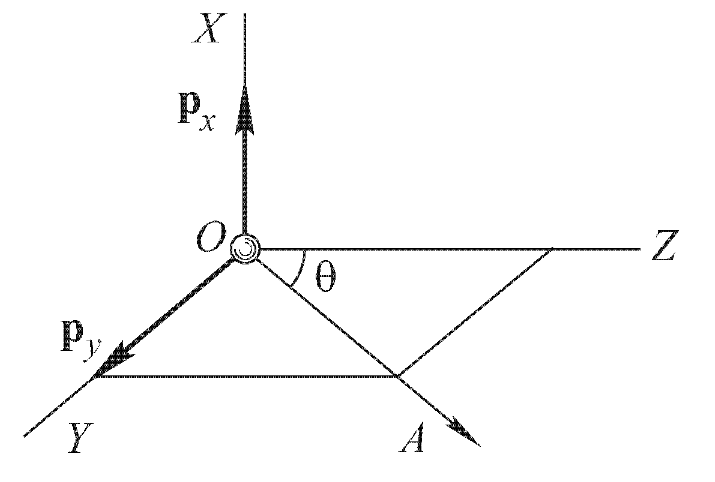
\includegraphics[width=0.25\textwidth]{figures/95_1.png}
    \caption{Рассеяние естественного света}
    \label{fig:freaky}
\end{figure}
Направим ось $X$ нормально к $OA$ и $OZ$, в силу $\vc{p} \parallel \vc{E}_0$ верно, что $\vc{p} \parallel XY$, тогда по найденному значению для $I_1$ с $\theta = \pi/2$ и $\theta = \pi/2- \vartheta$, можем найти интенсивности дипольных моментов $\vc{p}_x$ и $\vc{p}_y$. В силу ествественности падающего света, эти излучения \textit{некогерентны}, точнее некогерентны интенсивности от $\vc{p}_x$ и $\vc{p}_y$:
\begin{equation*}
    I_{1, \smallvc{p}_x} = 9 \varepsilon_0^2 \left(
        \frac{\varepsilon-\varepsilon_0}{\varepsilon+2 \varepsilon_0}
    \right)^2 \frac{\pi^2 V_1^2}{\lambda^4} \frac{\sin^2 \pi/2}{r^2} I_0,
    \hspace{10 mm} 
    I_{1, \smallvc{p}_y} = 9 \varepsilon_0^2 \left(
        \frac{\varepsilon-\varepsilon_0}{\varepsilon+2 \varepsilon_0}
    \right)^2 \frac{\pi^2 V_1^2}{\lambda^4} \frac{\cos^2 \vartheta}{r^2} I_0,
\end{equation*}
так что их можно просто сложить, тогда получим
\begin{equation*}
     I_1 
     =
    \frac{\omega^4}{4 \pi \varepsilon_0 v^3 r^2} \left(
        \overline{p_x^2} + \overline{p_y^2} \cos^2 \vartheta
     \right) 
     = 
     \frac{\omega^4}{4 \pi \varepsilon_0 v^3 r^2} \frac{1+\cos^2 \vartheta}{2} \overline{p^2} 
     =
     9 \varepsilon_0^2 \fbr{\varepsilon-\varepsilon_0}{\varepsilon+2 \varepsilon_0}^2 \frac{\pi^2 V_1^2}{\lambda^4} \frac{1+\cos^2 \theta}{2 r^2} I_0,
 \end{equation*} 
 где учтено $\overline{p_x^2} = \overline{p_y}^2 = \frac{1}{2} \overline{p^2}$. 
 а формула для $\mathcal P_1$ останется без изменений. 




\textbf{Частично поляризованный свет}. Полная линейная поляризация наблюдается только при $OA \bot $ направлению распространения падающего света, так как тогда $\vc{p}_y$ не даёт излучения. 


Если же посчитать интенсивность $I$ света, рассеиваемого объемом $V$, содержащим много шариков $\sub{N}{шар} V$, то, складывая интенсивности и рассматривая $r^3 \gg V$, найдём
\begin{equation*}
    I = 9 \varepsilon_0^2 \fbr{\varepsilon-\varepsilon_0}{\varepsilon+2 \varepsilon_0}^2
    \pi^2 \frac{V_1^2}{\lambda^4} \frac{1+\cos^2 \theta}{2 r^2} N V I_0.
\end{equation*}
Эта формула была получена Рэлеем, и по ней $I \sim \omega^{-4}$, что называют \textit{законом Рэлея}, что справедливо для сред с частицами, размеры которых малы по сравнению с длиной волны. 



\textbf{Убывание интенсивности}. Выделим цилиндр $\parallel OZ$ и рассмотрим баланс $I_0 (z) - I_0 (z+\d z) = \d I_0 = \mathcal P_1 N \d z$, тогда
\begin{equation*}
    \d I_0 = - \gamma I_0 \d z, \hspace{10 mm} 
    \gamma = 24 \pi^3 \varepsilon_0^2 \fbr{\varepsilon-\varepsilon_0}{\varepsilon+2 \varepsilon_0}^2 \frac{N V_1^2}{\lambda^4},
    \hspace{0.5cm} \Rightarrow \hspace{0.5cm}
    I_0 = \const \cdot e^{- \gamma z},
\end{equation*}
где $\gamma$ -- \textit{коэффициент рассеяния}.


\textbf{Молекулярное рассеяние (рассеяние Рэлея)}. 
Стоит заметить, что в атмосфере рассеяние происходит не посторонними частицами, а самими \textit{молекулами воздуха}. Такое рассеяние света называется \textit{рэлеевским} или \textit{молекулярным рассеянием}. На самом деле\footnote{
    1908 г., М. Смолуховский.
}  молекулярное рассеяние вызывается тепловым флуктуациями показателя преломления, которые и делают среду оптически мутной. 


Среда разбивается на $dV \ll \lambda^3$, при этом $N \d V \gg 1$. 
Уравнения на $\vc{H}'$ и $\vc{E}'$ остаются верны, последовательными приближениями можем получить
\begin{equation*}
    \delta \vc{P} = \frac{\delta \varepsilon}{4\pi} \vc{E}_0,
    \hspace{5 mm} 
    \vc{p} = \frac{\delta_i \varepsilon \cdot \delta_i V}{4 \pi} \vc{E}_0.
\end{equation*}
Это выражение отличается от случая с <<шариками>> только коэффициентом, так что верно, что
\begin{equation*}
    I_i = \frac{\pi^2}{\lambda^4} \frac{1 + \cos^2 \theta}{2 r^2} I_0 (\delta_i V)^2 \overline{(\delta_i \varepsilon)^2}.
\end{equation*}

Так, например, в случае идеального газа, верна формула
\begin{equation*}
    \varepsilon_i = 1 + 4 \pi \beta \frac{N_i}{\delta_i V},
\end{equation*}
где $\beta$ -- поляризуемость молекулы, а $N_i$ -- число молекул в $\delta_i V$. Так как $\delta_i V$ фиксирован, то $\delta_i \delta \varepsilon_i = 4 \pi \beta \delta N_i$, т.е. рассеяние вызывается \textit{флуктуациями числа молекл} в $\delta_i V$.


% см. 638 Сивухина
Аккуратно работая с этими флуктуациями, можем получить \textit{формулу Рэлея}:
\begin{equation*}
    I = \frac{2\pi^2}{\lambda^4} \frac{V}{N} (n-1)^2 \frac{1+\cos^2 \theta}{r^2} I_0,
\end{equation*}
что верно для изотропных молекул.


Для неидеальных газов и жидкостей можно получить формулу, вида
\begin{equation*}
    I = \frac{\pi^2}{\lambda^4} \frac{1+\cos^2 \theta}{2 r^2} V  I_0 \cdot
    \left(\rho \frac{d \varepsilon}{d \rho} \right)^2 \frac{kT}{(- v \partial_v P)_T},
\end{equation*}
полученную Эйнштейном в 1910 г. 





